\documentclass{article}


%\usepackage[final]{nips_anon}

\usepackage[table]{xcolor}
\usepackage[utf8]{inputenc}
\usepackage{textcomp}
\usepackage{amsmath}
\usepackage{dsfont}
\usepackage{listings}
\usepackage{amsfonts}
\usepackage{amssymb}
\usepackage{tabularx}
\usepackage{booktabs}
\usepackage{enumitem}
\usepackage{algorithm}% http://ctan.org/pkg/algorithm
\usepackage[noend]{algorithmic}
\usepackage{parskip}
\usepackage{tikz}
\usepackage[margin=1in]{geometry}
\usepackage{graphicx}
\usepackage{hyperref}
\usepackage{epigraph}
\usetikzlibrary{arrows,fit,positioning}
\usepackage{subcaption}
\usepackage[colorinlistoftodos]{todonotes}
\usepackage[numbers]{natbib} %numbers
\usepackage{wrapfig}
\usepackage{centernot}

% this is included to get tables with colored rows to not draw over hlines and vlines
\usepackage{etoolbox}

\makeatletter
\patchcmd{\@classz}
  {\CT@row@color}
  {\oldCT@column@color}
  {}
  {}
\patchcmd{\@classz}
  {\CT@column@color}
  {\CT@row@color}
  {}
  {}
\patchcmd{\@classz}
  {\oldCT@column@color}
  {\CT@column@color}
  {}
  {}
\makeatother


\usepackage{amsthm}

\graphicspath{ {figures/} }
\pgfarrowsdeclarecombine{ring}{ring}{}{}{o}{o}

\DeclareMathOperator{\ringarrow}{\raisebox{0.5ex}{\tikz[baseline]{\draw[ring->](0,0)--(2em,0);}}}
\DeclareUnicodeCharacter{00A0}{ }




\tikzset{
    %Define standard arrow tip
    >=stealth',
    %Define style for boxes
    punkt/.style={
           circle,
           rounded corners,
           draw=black, thick,
           text width=1em,
           minimum height=1em,
           text centered},
    observed/.style={
           circle,
           rounded corners,
           draw=black, thick,
           minimum width=2.3em,
           minimum height=2.3em,
           font=\footnotesize,
           text centered,
           fill=black!10!white
           },
     latent/.style={
           circle,
           rounded corners,
           draw=black, thick, dashed,
           minimum width=2.2em,
           minimum height=2.2em,
           font=\footnotesize,
           text centered
           },
    target/.style={
           circle,
           rounded corners,
           draw=black, thick,
           minimum width=2.2em,
           minimum height=2.2em,
           font=\footnotesize,
           text centered,
           fill=black!20!white,
           },
    observedrect/.style={
           rectangle,
           rounded corners,
           draw=black, thick,
           minimum width=6em,
           minimum height=2em,
           font=\footnotesize,
           text centered,
           fill=black!10!white
           },
    latentrect/.style={
           rectangle,
           rounded corners,
           draw=black, thick, dashed,
           minimum width=2.2em,
           minimum height=2.2em,
           font=\footnotesize,
           text centered
           },
     targetrect/.style={
           rectangle,
           rounded corners,
           draw=black, thick,
           minimum width=6em,
           minimum height=2em,
           font=\footnotesize,
           text centered,
           fill=black!20!white,
           },
     empty/.style={
           circle,
           rounded corners,
           minimum width=.5em,
           minimum height=.5em,
           font=\footnotesize,
           text centered,
           },
    % Define arrow style
    pil/.style={
           o->,
           thick,
           shorten <=2pt,
           shorten >=2pt,},
    sh/.style={ shade, shading=axis, left color=red, right color=green,
    shading angle=45 }   
}





\newcommand{\KL}{\operatorname{KL}}

\newcommand{\Pij}[1]{\operatorname{P}_{ij}\!\left\{#1\right\}}
\newcommand{\Pkl}[1]{\operatorname{P}_{kl}\!\left\{#1\right\}}
\newcommand{\Q}[1]{\operatorname{Q}\left(#1\right)}
\newcommand{\EE}{\mathbb E}
\newcommand{\EEa}{\EE_a}
\newcommand{\Pns}[2]{\operatorname{P}_{#1}\left\{#2\right\}}
\newcommand{\Pn}[2]{\operatorname{P}\left\{#2|#1\right\}}
\newcommand{\actions}{\mathcal{A}}
\newcommand{\calA}{\mathcal A}
\newcommand{\etc}{\textit{etc}}
\newcommand{\ie}{\textit{i.e.}}
\newcommand{\eg}{\textit{e.g.}}
\newcommand{\calP}{\mathcal P}
\newcommand{\x}{\boldsymbol{x}}
\newcommand{\Ps}{\operatorname{P}}
\newcommand{\R}{\mathbb R}
\newcommand{\Pri}[1]{\operatorname{P}_i\left\{#1\right\}}
\newcommand{\Prz}[1]{\operatorname{P}_0\left\{#1\right\}}
\newcommand{\indep}[1]{\mathcal{I}\left(#1\right)}
\newcommand{\vb}[1]{\boldsymbol{#1}}
\newcommand{\card}[1]{\left\vert{#1}\right\vert}
\newcommand{\actionspace}{\mathcal{A}}



\newcommand{\Esub}[2]{\mathbb E_{#1}\left[{#2}\right]}
\newcommand{\defined}{\vcentcolon =}
\newcommand{\rdefined}{=\vcentcolon}
\newcommand{\E}[1]{\mathbb E\left[{#1}\right]}
\newcommand{\Var}{\operatorname{Var}}
\newcommand{\calF}{\mathcal F}
\newcommand{\sr}[1]{\stackrel{#1}}
\newcommand{\set}[1]{\left\{#1\right\}}
\newcommand{\ind}[1]{\mathds{1}\!\!\set{#1}}

\newcommand{\argmax}{\operatornamewithlimits{arg\,max}}
\newcommand{\argmin}{\operatornamewithlimits{arg\,min}}
\newcommand{\floor}[1]{\left \lfloor {#1} \right\rfloor}
\newcommand{\ceil}[1]{\left \lceil {#1} \right\rceil}
\newcommand{\eqn}[1]{\begin{align}#1\end{align}}
\newcommand{\eq}[1]{\begin{align*}#1\end{align*}}
\newcommand{\Ber}{\operatorname{Bernoulli}}
\newcommand{\bigo}[1]{\mathcal{O}\left( #1 \right)}
\newcommand{\bigotilde}[1]{\tilde{\mathcal{O}}\left( #1 \right)}
\newcommand{\bigtheta}[1]{\Theta\left( #1 \right)}
\newcommand{\bigthetatilde}[1]{\tilde{\Theta}\left( #1 \right)}
\newcommand{\bigomega}[1]{\Omega\left( #1 \right)}

\renewcommand{\P}[1]{\operatorname{P}\left(#1\right)}
\newcommand{\cf}[2]{{#1}^{#2}}
\newcommand{\cfb}[2]{{#1}_t^{#2}} % used to represent reward
\newcommand{\bernoulli}{\operatorname{Bernoulli}}
\newcommand{\dirac}{\operatorname{Dirac}}
\newcommand{\parents}[1]{\operatorname{\mathcal{P}a}_{#1}}
\renewcommand{\vec}[1]{\boldsymbol{#1}}
\newcommand{\regret}{\bar{R}_{T}} %psuedo-regret
\newcommand{\expectedregret}{\mathbb{E}R_{T}} % expected regret
\newcommand{\rawregret}{R_{T}} % plain regret
\newcommand{\simpleregret}{R_T}
\newcommand{\quotes}[1]{``#1''}

\theoremstyle{plain} 
\newtheorem{theorem}{Theorem}
\newtheorem{proposition}[theorem]{Proposition}
\newtheorem{lemma}[theorem]{Lemma}
\newtheorem{corollary}[theorem]{Corollary}

\theoremstyle{definition}
\newtheorem{definition}[theorem]{Definition}
\newtheorem{assumption}[theorem]{Assumption}
\newtheorem{remark}[theorem]{Remark}
\newtheorem{example}[theorem]{Example}
\let\temp\epsilon
\let\epsilon\varepsilon

\newcommand{\ci}{\mathrel{\perp\mspace{-10mu}\perp}}
\newcommand{\nci}{\centernot{\ci}}


\title{Causal Bandits: Learning Good Interventions via Causal Inference}

% The \author macro works with any number of authors. There are two
% commands used to separate the names and addresses of multiple
% authors: \And and \AND.
%
% Using \And between authors leaves it to LaTeX to determine where to
% break the lines. Using \AND forces a line break at that point. So,
% if LaTeX puts 3 of 4 authors names on the first line, and the last
% on the second line, try using \AND instead of \And before the third
% author name.
\author{
  Finnian Lattimore \\
  Australian National University and Data61/NICTA \\
  \texttt{finn.lattimore@gmail.com} \\
   \and
   Tor Lattimore \\
   University of Alberta \\
  \texttt{tor.lattimore@gmail.com} \\
   \and
   Mark D. Reid \\
   Australian National University and Data61/NICTA \\
   \texttt{mark.reid@anu.edu.au} \\
}


\begin{document}

\maketitle

\begin{abstract} 
We study the problem of using causal models to improve the rate at which good interventions can be learned online in a stochastic environment. 
Our formalism combines multi-arm bandits and causal inference to model a novel type of bandit feedback that is not exploited by existing approaches.
We propose a new algorithm that exploits the causal feedback and prove a bound on its simple regret that is strictly better (in all quantities) 
than algorithms that do not use the additional causal information. This is an extended version of our paper published in NIPS 2016, \citet{NIPS2016_6195}.
\end{abstract} 

\section{Introduction}
\label{sec:intro_causal_bandit}

Medical drug testing, policy setting, and other scientific processes are commonly framed and analysed in the language of sequential experimental design and, in special cases, as bandit problems~\citep{Robbins1952,Chernoff1959}. 
In this framework, single actions (also referred to as interventions) from a pre-determined set are repeatedly performed in 
order to evaluate their effectiveness via feedback from a single, real-valued reward signal.
We propose a generalisation of the standard model by assuming that, in addition to the reward signal, the learner observes the values of a number of covariates 
drawn from a probabilistic causal model~\citep{Pearl2000}.
Causal models are commonly used in disciplines where explicit experimentation may be difficult such as social science, demography and economics.
For example, when predicting the effect of changes to childcare subsidies on workforce participation, or school choice on grades. 
Results from causal inference relate observational distributions to interventional ones, allowing the outcome of an intervention to be predicted without
explicitly performing it.
By exploiting the causal information we show, theoretically and empirically, how non-interventional observations can be used to improve the rate at 
which high-reward actions can be identified.

The type of problem we are concerned with is best illustrated with an example. 
Consider a farmer wishing to optimise the yield of her crop. 
She knows that crop yield is only affected by temperature, a particular soil nutrient, and moisture level but the precise effect of their combination is unknown.
In each season the farmer has enough time and money to intervene and control at most one of these variables:
deploying shade or heat lamps will set the temperature to be low or high; the nutrient can be added or removed through a choice of fertilizer; and irrigation or rain-proof covers will keep the soil wet or dry.
When not intervened upon, the temperature, soil, and moisture vary naturally from season to season due to weather conditions and these are all observed along with the final crop yield at the end of each season.
How might the farmer best experiment to identify the single, highest yielding intervention in a limited number of seasons?
%without sacrificing too much crop yield (relative to always choosing the best intervention) in the process?

\paragraph{Contributions} We take the first step towards formalising and solving problems such as the one above. 
In \S\ref{sec:setup-defs} we formally introduce \emph{causal bandit problems} in which interventions are treated as arms in a bandit problem but their influence on the reward --- along with any other observations --- is assumed to conform to a known causal graph. 
We show that our causal bandit framework subsumes the classical bandits (no additional observations) and contextual stochastic bandit problems (observations are revealed before an intervention is chosen) before focusing on the case where, like the above example, observations occur \emph{after} each intervention is made.

Our focus is on the simple regret, which measures the difference between the return of the optimal action and that of the action chosen by the algorithm after $T$ rounds.
In \S\ref{sec:simple-regret} we analyse a specific family of causal bandit problems that we call \emph{parallel bandit} problems in which $N$ factors affect the reward independently and there are $2N$ possible interventions.
We propose a simple causal best arm identification algorithm for this problem and show that up to logarithmic factors it enjoys minimax optimal
simple regret guarantees of $\smash{\tilde\Theta(\sqrt{m/T})}$ where $m$ depends on the causal model and may be much smaller than $N$.
In contrast, existing best arm identification algorithms suffer $\smash{\Omega(\sqrt{N/T})}$ simple regret (Thm. 4 by \citet{audibert2010best}).
This shows theoretically the value of our framework over the traditional bandit problem. 
Experiments in \S\ref{sec:experiments} further demonstrate the value of causal models in this framework.

In the general casual bandit problem interventions and observations may have a complex relationship. 
In \S\ref{sec:simple-regret-general} we propose a new algorithm inspired by importance-sampling that a) enjoys sub-linear regret equivalent 
to the optimal rate in the parallel bandit setting and b) captures many of the intricacies of sharing information in a causal graph in the general case.
As in the parallel bandit case, the regret guarantee scales like $\smash{O(\sqrt{m/T})}$ where $m$ depends on the underlying causal structure, with 
smaller values corresponding to structures that are easier to learn. The value of $m$ is always less than the number of interventions $N$ and in the special
case of the parallel bandit (where we have lower bounds) the notions are equivalent.

\section{Problem Setting}
\label{sec:setup-defs}

A natural way to connect the causal framework with the bandit setting is to model the action space as interventions on variables in a causal directed acyclic graph. Each possible assignment of variables to values is a potential action (or bandit arm), see figure \ref{fig:unify_frameworks} for a simple example. In some settings, it makes sense to restrict the action space available to the agent to a subset of all the possible actions, for example the set of single variable interventions. The reward could be a general function of the action selected and the final state of the graph. However for simplicity, we will consider the reward to be the value of a single specified node. We refer to these problems as \emph{causal bandit problems}. In this paper we focus on the case where the causal graph is known. Extending this work to simultaneously learning the casual graph is discussed in \S\ref{sec:causal_bandit_discussion}.

\begin{figure}
\centering
\begin{subfigure}[c]{0.3\textwidth}
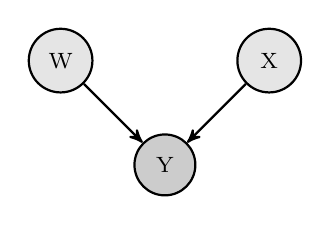
\begin{tikzpicture}[->,shorten >=0pt,shorten <=0pt,node distance=3em,thick,main node/.style={observed}, tg/.style={target}]
\node[main node](1){W};
\node[tg, below right=of 1](2){Y};
\node[main node, above right=of 2](3){X};
\path[]
	(1) edge (2)
	(3) edge (2);
\end{tikzpicture}
\end{subfigure}
\begin{subfigure}[t]{0.4\textwidth}
$\actionspace$ = \begin{tabular}{|c|}
	\hline
  $do(W=0,Z=0)$ \\
  $do(W=0,Z=1)$ \\
  $do(W=1,Z=0)$ \\
  $do(W=1,Z=1)$ \\
  \hline
  $do(W=0)$ \\
  $do(W=1)$ \\
  $do(Z=0)$ \\
  $do(Z=1)$ \\
  $do()$ \\
  \hline
\end{tabular}
\end{subfigure}
\caption{A simple causal graphical model and corresponding complete action space. $W$ and $Z$ represent binary variables that can be intervened on and $Y$ represents the reward.}
\label{fig:unify_frameworks}
\end{figure} 


We will assume each variable only takes on a finite number of distinct values. (The path to relaxing this assumption would be through levering the work on continuous armed bandits). The \emph{parents} of a variable $X_i$, denoted $\parents{X_i}$, is the set of all variables $X_j$ such that there is an edge from $X_j$ to $X_i$ in $\mathcal{G}$. An \emph{intervention or action (of size $n$)}, denoted $do(\vec{X}=\vec{x})$, assigns the values $\vec{x}=\{x_1, \ldots, x_n\}$ to the corresponding variables $\vec{X}=\{X_1, \ldots, X_n\} \subset \mathcal{X}$ with the empty intervention (where no variable is set) denoted $do()$. We denote the expected reward for the action $a = do(\vec{X} = \vec{x})$ by $\mu_{a} := \E{Y | do(\vec{X} = \vec{x})}$ and 
the optimal expected reward by $\mu^* := \max_{a\in\actions} \mu_{a}$. 

\vspace*{.5cm}
\begin{definition}[Causal bandit problem]
A learner for a casual bandit problem is given the casual model’s graph $G$ over variables $\mathcal{X}$ and a set of allowed actions $\actionspace$. Each action $a \in \actionspace$ assigns a value to a subset of the variables in $\mathcal{X}$ and incurs a known cost $C(a)$ on the learner. One variable $Y \in \mathcal{X}$ is designated as the \emph{reward variable}.

The causal bandit game proceeds over $T$ rounds. In each round $t$, the learner:
\begin{enumerate}
\item \emph{observes} the value of a subset of the variables $\vec{X}^c_t$,
\item \emph{intervenes} by choosing $a_t = do(\vec{X}_t = \vec{x}_t) \in \mathcal{A}$ based on previous observations and rewards, 
\item \emph{observes} values for another subset of variables $\vec{X}^o_t$ drawn from $\P{\vec{X}^o_t |\vec{X}^c_t, do(\vec{X}_t = \vec{x}_t)}$,
\item \emph{obtains reward} $r_t = Y_t - C(a_t)$, where $Y_t$ is sampled from $\P{Y_t| \vec{X}^c_t, do(\vec{X}_t = \vec{x}_t)}$
\end{enumerate} 
\end{definition}

We refer to the set of variables that can be observed prior to selecting an action $\vec{X}^c$ as contextual variables and the set of variables observed after the action is chosen, $\vec{X}^o$, as post-action feedback variables. Note that $\vec{X}^c$ and $\vec{X}^o$ need not be disjoint. A variable may be observed both prior to and after the agent selects an action, and the action may change its value. The notation $\P{\cdot|\vec{X}^c_t, do(\vec{X}_t = \vec{x}_t)}$ denotes distributions conditional on having observed $\vec{X}^c_t$ and \emph{then} intervened to set $\vec{X}_t = \vec{x}_t$. The values of variables in $\vec{X}^c_t$ that are non-decendents of $\vec{X}_t$ remain unchanged by the intervention. The objective of the learner is to minimise either the simple or cumulative regret. 

The causal bandit problem takes on characteristics of different bandit settings depending on the action-space $\actionspace$ and correspondign costs, which variables are observable prior to selecting an action and on which variables we receive post-action feedback. If we can (cheaply) intervene on all of the parents of $Y$ simultaneusly then any context or alternative actions are irrelevent and the problem reduces to a standard multi-armed bandit problem. This is formalised in theorem \ref{theorem:cb-intervene-all-parents}. 

\vspace{0.5cm}
\begin{theorem}
\label{theorem:cb-intervene-all-parents}
Let $\mathcal{A'}$ be the set of all possible assignments of values to the parents of $Y$. If $\mathcal{A'} \subseteq \mathcal{A}$ and $C(a') \leq C(a) \; \forall (a' \in \mathcal{A'}, a \in \mathcal{A}/\mathcal{A'})$ then the optimal action $a^* \in \mathcal{A'}$ and the problem reduces to a standard multi-armed bandit (over actions in in $\mathcal{A'}$).
\begin{proof}
for any action $a \in \mathcal{A}$, 
\eq{
 \E{Y|\vec{X}^c_t,a} &= \Esub{\parents{Y}\sim \P{\parents{Y}|\vec{X}^c_t,a}}{\E{Y|\vec{X}^c_t,a,\parents{Y}}} \\
 &= \Esub{\parents{Y}\sim \P{\parents{Y}|\vec{X}^c_t,a}}{\E{Y|\parents{Y}}}\\
 &= \Esub{\parents{Y}\sim \P{\parents{Y}|\vec{X}^c_t,a}}{\E{Y|do(\parents{Y})}}\\
 &\leq \max_{\parents{Y}}\E{Y|do(\parents{Y})} = \E{Y|a'} \text{ for some $a' \in \mathcal{A'}$}
}
\end{proof}
\end{theorem} 


If feedback is received only on the reward node $\vec{X}^o = \set{Y}$, as in the standard bandit setting, then the do-calculus can be applied to eliminate some actions immediately, before any experiments are performed and then a standard bandit algorithm can be run on the remaining actions, see figure \ref{fig:cholesterol_graph} as an example. If we receive post-action feedback on additional nodes the problem can be more interesting. In addition to being able to eliminate some actions prior to sampling any data as in the previous case, taking one action may give us some information on actions that were not selected. Consider again the model in figure \ref{fig:unify_frameworks}. The causal structure implies: 

\eq{
P(Y|do(W = 0)) &= P(Y|do(),W = 0) \\
&= P(Y|do(X=0),W=0)P(X=0)+P(Y|do(X=1),W=0)P(X=1) 
}

\begin{figure}
\centering
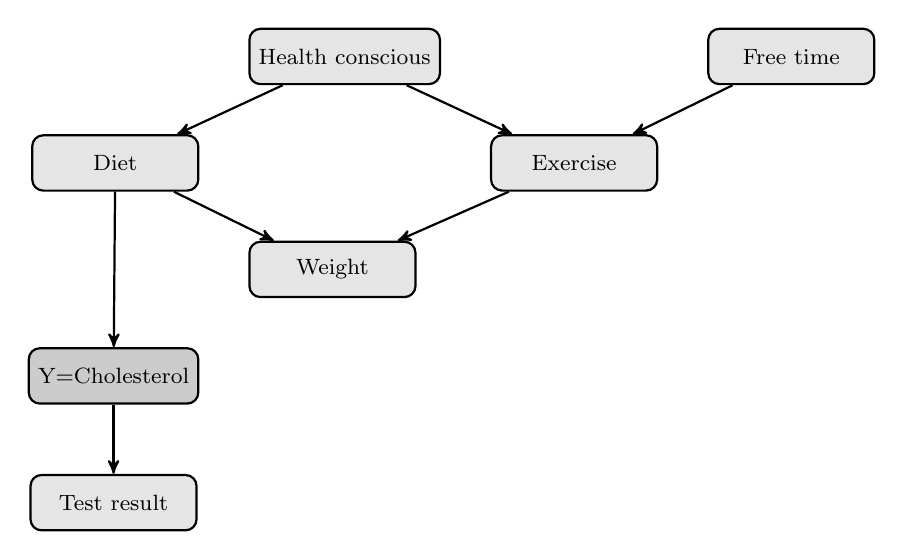
\begin{tikzpicture}[->,shorten >=0pt,shorten <=0pt,node distance=2.5em,thick,node/.style={observedrect},tg/.style={targetrect}]
\node[node](1){Health conscious};
\node[node, below left=of 1](2){Diet};
\node[node, below right=of 1](3){Exercise};
\node[node, below right=of 2](4){Weight};
\node[tg,below left=of 4](5){Y=Cholesterol};
\node[node, below =of 5](6){Test result};
\node[node, above right=of 3](7){Free time};
\path[]
	(1) edge (2) edge (3)
	(2) edge (4) edge (5)
	(3) edge (4)
	(5) edge (6)
	(7) edge (3);
\end{tikzpicture}
\caption{Example causal graph (based on \citet{Koller2009}) where the outcome of interest (reward) is cholesterol level . The do-calculus can be applied to eliminate some actions immediately without the need to do any experiments. For example, no actions involving 'Test Result' need to be considered and interventions on 'Diet' do not need to be considered in conjunction with any other variables.}
\label{fig:cholesterol_graph}
\end{figure}

Thus we gain information about the reward for the action $do(W=0)$ from selecting the action $do()$ or $do(X = x)$ and then observing $W = 0$.  We only get this form of side information for actions that don't specify the value of every variable, for example those in the bottom half of the table in figure \ref{fig:unify_frameworks}. If additional variables are only observed before an intervention is selected the causal bandit problem can be treated as a stochastic contextual bandit problem, which are already reasonably well understood \citep{Agarwal2014}.

Two other problems that sit in the space between causal inference and bandit problems, bandits with unobserved confounders \cite{Bareinboim2015} and compliance aware bandits \citep{DellaPenna2016}, can also be viewed as specific causal bandit problems. In the work on bandits with unobserved confounders it is assumed that the reward given each action may depend on some latent variable $U$ which we cannot observe directly. However, prior to selecting an action, we can observe  $I$, the action that would have been selected under an alternate (stationary) policy, which may depend on $U$, see figure \ref{fig:confounded-causal-bandit-graph}. In this case the set of contextual variables $\vec{X}^c = I$, the set of post-action feedback variables $\vec{X}^o = \set{Y}$ and the action space consists of all possible assigments of values to a single node $X$, $\actionspace = do(X=x)$. This setting reduces to a contextual bandit problem in our causal bandit framework. However in thier work on bandits with unobserved confounders \citet{Forney2017} also leverage the fact that $I$ represents the action that would have been selected under an alternate policy to fuse data collected under the previous (observational) policy with data collected under the new policy. This information is not encoded in the causal bandit graph in figure \ref{fig:confounded-causal-bandit-graph}, as $I$ could be any variable that is influenced by the unobserved context $U$, and thus cannot be exploited by a standard contextual bandit algorithm. 

Compliance aware bandits describe situations in which the action recommended by the bandit algorithm is not always followed. For example a patient may refuse to take a treatment or an advertiser may have complex rules about how many ads a given customer can recieve which prevends some of the suggestions from the ad recomendation engine from being followed. After an action is selected the algorithm can observe the action that was actually taken in addition to the reward. \citet{DellaPenna2016} analyse this setting with binary treatments both with and without the presense of a latent confounding variable $U$, see figure \ref{fig:imperfect-compliance-causal-bandit-graph}. In this case, there are no contextual variables and the action space is again the set of assignments to a single variable but there is post-action feedback, which reveals the value of the action that was actually taken.\footnote{There are some interesting variants of the compliance aware bandit setting that, to my knowledge, have not been analysed. The first is if the confounding variable $U$ is observable, either as context or post-action feedback. The second is if we extend the allowable action set to include acting directly on $X$, albeit at a higher cost than acting on $A$. It is also worth noting the connection between this setting and instrumental variables \cite{balke1997bounds}. By making some functional assumptions about the relationships between the variables, we can use $A$ as an instrumental variable to bound or estimate the (casual) effect of $X$ on $Y$. The estimation will be somewhat complicated in the bandit setting because the action chosen at each timestep is dependent on the previous sequence actions and rewards.}

\begin{figure}[h]
\centering
\begin{subfigure}[t]{0.49\textwidth}
\centering
\caption{Bandits with unobserved confounders:$\vec{X}^c=\set{I}$, $\vec{X}^o = \set{Y}$, $\actionspace = do(X=x)$}
\label{fig:confounded-causal-bandit-graph}
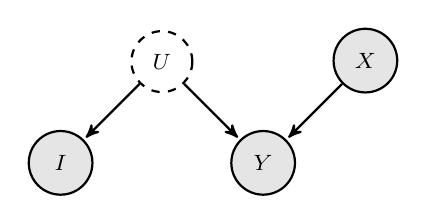
\begin{tikzpicture}[->,>=stealth',shorten >=1pt,auto,node distance=1cm,
  thick,main node/.style={observed},lt/.style={latent}]
 %nodes
\node[lt](1){${U}$};
\node[main node, below right =of 1](2){${Y}$};
\node[main node, below left=of 1](3){$I$};
\node[main node, above right=of 2](4){$X$};
 \path[every node/.style={font=\sffamily\small}]
   (1) edge (2) edge (3)
   (4) edge (2);
\end{tikzpicture} 
\end{subfigure}
\begin{subfigure}[t]{0.49\textwidth}
\centering
\caption{Compliance aware bandits: $\vec{X}^c=\set{}$, $\vec{X}^o = \set{T,Y}$, $\actionspace = do(X=x)$ }
\label{fig:imperfect-compliance-causal-bandit-graph}
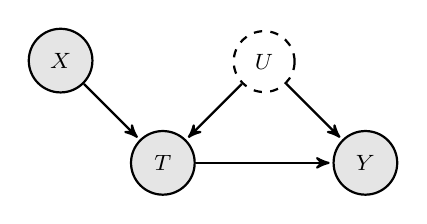
\begin{tikzpicture}[->,>=stealth',shorten >=1pt,auto,node distance=1cm,
  thick,main node/.style={observed},lt/.style={latent}]
 %nodes
\node[lt](1){$U$};
\node[main node, below left=of 1](2){$T$};
\node[main node, below right=of 1](3){$Y$};
\node[main node, above left=of 2](4){$X$};
 \path[every node/.style={font=\sffamily\small}]
   (1) edge (2) edge (3)
   (2) edge (3)
   (4) edge (2);
\end{tikzpicture} 
\end{subfigure}
\caption{}
\label{fig:causal-bandit-version-confounded-compliance}
\end{figure}

The classical $K$-armed stochastic bandit problem can be recovered in our framework by considering a simple causal model with one edge connecting a single variable $X$ that can take on $K$ values to a reward variable $Y \in \set{0,1}$ where $\P{Y = 1|X} = r(X)$ for some arbitrary but unknown, real-valued function $r$. The set of allowed actions in this case is $\mathcal{A} = \{ do(X = k) \colon k \in \{1, \ldots, K\}\}$. Conversely, any causal bandit problem can be reduced to a classical stochastic $|\mathcal{A}|$-armed bandit problem by treating each possible intervention as an independent arm and ignoring all sampled values for the observed variables except for the reward. However, the number of actions or arms grows exponentially with the number of variables in the graph making it important to develop algorithms that leverage the graph structure and additional observations.

\paragraph{Related Work} As alluded to above, causal bandit problems can be treated as classical multi-armed bandit problems by simply ignoring the causal model and extra observations and applying an existing best-arm identification algorithm with well understood simple regret guarantees \citep{Jamieson2013}. However, as we show in \S\ref{sec:simple-regret}, ignoring the extra information available in the non-intervened variables yields sub-optimal performance.

Our framework bears a superficial similarity to contextual bandit problems, since the extra observations on non-intervened variables might be viewed as context for selecting an intervention. 
However, a crucial difference is that in our model the extra observations are only revealed \emph{after} selecting an intervention and hence cannot be used as context. 

There have been several proposals for bandit problems where extra feedback is received after an action is taken.
Most recently, \citet{Alon2015}, \citet{Kocak2014} have considered very general models related to partial monitoring games~\citep{Bartok2014} where rewards on un-played actions are revealed according to a feedback graph. As we discuss in \S\ref{sec:causal_bandit_discussion}, the parallel bandit problem can be captured in this framework, however the regret bounds are not optimal in our setting. They also focus on cumulative regret, which cannot be used to guarantee low simple regret~\citep{Bubeck2009a}. The partial monitoring approach taken by \citet{wu2015online} could be applied (up to modifications for the simple regret) to the parallel bandit, but the resulting strategy would need to know the likelihood of each factor in advance, while our strategy learns this online. \citet{Yu2009} utilise extra observations to detect changes in the reward distribution, whereas we assume fixed reward distributions and use extra observations to improve arm selection. \citet{Avner2012} analyse bandit problems where the choice of arm to pull and arm to receive feedback on are decoupled. The main difference from our present work is our focus on simple regret and the more complex information linking rewards for different arms via causal graphs. To the best of our knowledge, our paper is the first to analyse simple regret in bandit problems with extra post-action feedback.


%\citet{Yu2009} consider bandit problems where a learner chooses an arm to play as well as set of arms to observe rewards for in a stochastic setting where the reward distributions can change infrequently and the aim is to minimize cumulative regret. They use extra observations to detect changes whereas we assume fixed reward distributions and use extra observations to improve arm selection.
% Partial monitoring is a very general framework for for decoupling the feedback from the action and reward. It can be used to classify problems into one of four categories, trivial with no regret, easy with $R_T = \bigthetatilde{\sqrt{T}}$ , hard with $R_T = \bigtheta{T^{2/3}}$ and hopeless with $R_T = \bigomega{T}$ \citep{Bartok2014}. Partial monitoring algorithms yield results that are optimal with respect the horizon $T$ but not other parameters, such as $K$, which is the key focus of incorporating causal structure. 

Two pieces of recent work also consider applying ideas from causal inference to bandit problems.
\citet{Bareinboim2015} demonstrate that in the presence of confounding variables the value that a variable would have taken had it not been 
intervened on can provide important contextual information. Their work differs in many ways. For example, the focus is on the cumulative regret and
the context is observed before the action is taken and cannot be controlled by the learning agent.  

%\todof{write one sentence to explain how their work is different to ours}

 \citet{Ortega2014thompson} present an analysis and extension of Thompson sampling assuming actions are causal interventions. Their focus is on causal induction (\ie, learning an unknown causal model) instead of exploiting a known causal model. Combining their handling of  causal induction with our analysis is left as future work.


The truncated importance weighted estimators used in \S\ref{sec:simple-regret-general} have been studied before in a causal framework by \citet{Bottou2013}, 
where the focus is on learning from observational data, but not controlling the sampling process. They also briefly discuss some of the issues 
encountered in sequential design, but do not give an algorithm or theoretical results for this case.

\section{Causal bandits with post action feedback}

We now focus on causal bandit problems with post-action feedback, in which the value of all the variables are observed after an intervention is selected, the cost of all allowable actions is equal and the goal of the learner is to minimise the simple regret. 




\subsection{The parallel bandit problem}
\label{sec:simple-regret}
In this section we propose and analyse an algorithm for achieving the optimal regret in a natural special case of the causal bandit problem which we call the {\it parallel bandit}.
It is simple enough to admit a thorough analysis but rich enough to model the type of problem discussed in \S\ref{sec:intro_causal_bandit}, including the farming example. It also suffices to witness the regret gap between algorithms that make use of causal models and those which do not.

The causal model for this class of problems has $N$ binary variables $\{ X_1, \ldots, X_N \}$ where each $X_i \in \{0,1\}$ are independent causes of a reward variable $Y \in \set{0,1}$, as shown in Figure~\ref{fig:parallel}. All variables are observable and the set of allowable actions are all size 0 and size 1 interventions: $\mathcal{A} = \set{do()} \cup \set{ do(X_i = j) \colon 1 \leq i \leq N \text{ and } j \in \set{0,1}}$

In the farming example from the introduction, $X_1$ might represent temperature (\eg, $X_1=0$ for low and $X_1=1$ for high). The interventions $do(X_1 = 0)$ and $do(X_1 = 1)$ indicate the use of shades or heat lamps to keep the temperature low or high, respectively.

\begin{figure}
    \begin{subfigure}[t]{0.34\textwidth}
	\centering   
	 \caption{Parallel graph}\label{fig:parallel} 
          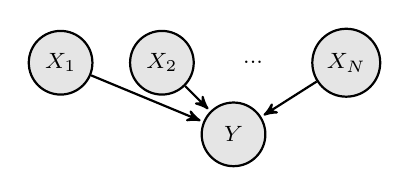
\begin{tikzpicture}[->,>=stealth',shorten >=1pt,auto,node distance=.45cm,
  thick,main node/.style={observed}, hidden/.style={empty},background rectangle/.style={fill=olive!45}]
%every node/.style={scale=0.6}
 %nodes
\node[main node](1){$X_{1}$};
\node[main node, right=of 1](2){$X_{2}$};
\node[hidden, right=of 2](3){$...$};
\node[main node, right=of 3](4){$X_{N}$};
\node[main node, below right=of 2](5){$Y$};
 \path[every node/.style={font=\tiny}]
    (1) edge (5)
    	(2) edge (5)
    (4) edge (5);
\end{tikzpicture} 
\end{subfigure}
    \begin{subfigure}[t]{0.25\textwidth}
    \centering
     \caption{Confounded graph}
        \label{fig:causalStructure_confounded}
        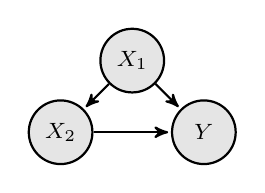
\begin{tikzpicture}[->,>=stealth',shorten >=1pt,auto,node distance=.45cm,
  thick,main node/.style={observed}, hidden/.style={empty},background rectangle/.style={fill=olive!45}]
\node[main node](1){$X_1$};
\node[main node, below left=of 1](2){$X_2$};
\node[main node, below right=of 1](4){$Y$};
 \path[every node/.style={font=\tiny}]
    (1) edge (2)
    (1) edge (4)
    (2) edge (4);
\end{tikzpicture}
    \end{subfigure}
    \begin{subfigure}[t]{0.4\textwidth}
    \centering
     \caption{Chain graph}
        \label{fig:causalchain}
         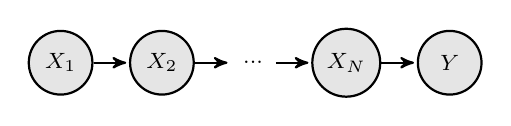
\begin{tikzpicture}[->,>=stealth',shorten >=1pt,auto,node distance=.45cm,
  thick,main node/.style={observed}, hidden/.style={empty},background rectangle/.style={fill=olive!45}]
\node[main node](1){$X_{1}$};
\node[main node, right=of 1](2){$X_{2}$};
\node[hidden, right=of 2](3){$...$};
\node[main node, right=of 3](4){$X_{N}$};
\node[main node, right=of 4](5){$Y$};
 \path[every node/.style={font=\tiny}]
    (1) edge (2)
  	(2) edge (3)
    (3) edge (4)
    (4) edge (5);
\end{tikzpicture}
    \end{subfigure}
      \caption{Causal Models}\label{fig:causalmodels}\label{fig:causal_models_causal_bandit}
\end{figure}


In each round the learner either purely observes by selecting $do()$ or sets the value of a single variable. The remaining variables are simultaneously set by independently biased coin flips. The value of all variables are then used to determine the distribution of rewards for that round. Formally, when not intervened upon we assume that each $X_i \sim \bernoulli(q_i)$ where $\vec{q} = (q_1, \ldots, q_N) \in [0,1]^N$ so that $q_i = \P{X_i = 1}$.

The value of the reward variable is distributed as $\P{Y = 1|\vec{X}} = r(\vec{X})$ where 
$r : \{0,1\}^N \to [0,1]$ is an arbitrary, fixed, and unknown function. 
In the farming example, this choice of $Y$ models the success or failure of a seasons crop, 
which depends stochastically on the various environment variables.


\paragraph{The Parallel Bandit Algorithm}
%\label{sub:par-bandit-alg}
The algorithm operates as follows. For the first $T/2$ rounds it chooses $do()$ to collect observational data. As the only link from each $X_1,\ldots,X_N$ to $Y$ is a direct, causal one, $\P{Y|do(X_i=j)}=\P{Y|X_i=j}$. Thus we can create good estimators for the returns of the actions $do(X_i = j)$ for which $\P{X_i = j}$ is large. The actions for which $\P{X_i = j}$ is small may not be observed (often) so  estimates of their returns could be poor. To address this, the remaining $T/2$ rounds are evenly split to estimate the rewards for these infrequently observed actions. The difficulty of the problem depends on $\vec{q}$ and, in particular, how many of the variables are unbalanced (\ie, small $q_i$ or $(1-q_i)$). For $\tau \in [2...N]$ let $I_\tau = \set{ i : \min\set{q_i, 1-q_i} < \frac{1}{\tau}}$. Define

\eq{
\label{eq:m-simple}
m(\vec{q}) = \min \set{ \tau : |I_{\tau}| \leq \tau}\,.
}


\begin{algorithm}[H]
\caption{Parallel Bandit Algorithm}\label{alg:simple}
\begin{algorithmic}[1]
\STATE {\bf Input:} Total rounds $T$ and $N$.
\FOR{$t \in 1,\ldots,T / 2$}
\STATE Perform empty intervention $do()$
\STATE Observe $\vec{X}_t$ and $Y_t$
\ENDFOR
\FOR{$a = do(X_i = x) \in \actions$}
\STATE Count times $X_i = x$ seen: $T_a = \sum_{t=1}^{T/2} \ind{X_{t,i} = x}$
\STATE Estimate reward: $\hat{\mu}_a = \frac{1}{T_a} \sum_{t=1}^{T/2} \ind{X_{t,i} = x} Y_t$ \\[0.2cm]
\STATE Estimate probabilities: $\hat{p}_a = \frac{2 T_a}{T}$,\,\, $\hat q_i = \hat p_{do(X_i = 1)}$
\ENDFOR
\STATE Compute $\hat{m} = m(\vec{\hat q})$ and $A = \set{a \in \actions \colon \hat{p}_a \leq \frac{1}{\hat m}}$.
\STATE Let $T_A := \frac{T}{2 |A|}$ be times to sample each $a\in A$.
\FOR{$a = do(X_i = x) \in A$}
\FOR{$t \in 1,\ldots,T_A$}
\STATE Intervene with $a$ and observe $Y_t$
\ENDFOR
\STATE Re-estimate $\hat{\mu}_a = \frac{1}{T_A} \sum_{t=1}^{T_A} Y_t$
\ENDFOR
\RETURN estimated optimal $\hat{a}^*_T \in \argmax_{a\in\actions} \hat{\mu}_a$
\end{algorithmic}
\end{algorithm}

$I_\tau$ is the set of variables considered unbalanced and we tune $\tau$ to trade off identifying the low probability actions against not having too many of them, so as to minimise the worst-case simple regret. When $\vec{q} = (\frac{1}{2}, \ldots, \frac{1}{2})$ we have $m(\vec{q}) = 2$ and when $\vec{q} = (0, \ldots, 0)$ we have $m(\vec{q}) = N$. We do not assume that $\vec{q}$ is known, thus Algorithm \ref{alg:simple} also utilises the samples captured during the observational phase to estimate $m(\vec{q})$. Although very simple, the following two theorems show that this algorithm is effectively optimal.


\begin{theorem}\label{thm:uq-simple}
Algorithm \ref{alg:simple} satisfies
\eq{
\simpleregret \in \bigo{\sqrt{\frac{m(\vec{q})}{T}\log\left(\frac{NT}{m(\vec{q})}\right)}}\,.
}
\end{theorem}


\begin{theorem}\label{thm:lower}
For all strategies and $T$, $\vec{q}$, there exist rewards such that
$\displaystyle \simpleregret 
\in \Omega\left(\sqrt{\frac{m(\vec{q})}{T}}\right)$.
\end{theorem}

The proofs of Theorems \ref{thm:uq-simple} and \ref{thm:lower} follow by carefully analysing the concentration
of $\hat p_a$ and $\hat m$ about their true values and may be found in Sections \ref{sec:thm:uq-simple} and \ref{sec:thm:lower} respectively.

%We prove a lower bound on the simple regret that matches up to logarithmic factors the upper bound given in Theorem \ref{thm:uq-simple}. 
By utilising knowledge of the causal structure, Algorithm \ref{alg:simple} effectively only has to explore the $m(\vec{q})$ 'difficult' actions. Standard multi-armed bandit algorithms must explore all $2N$ actions and thus achieve regret  $\smash{\Omega(\sqrt{N/T})}$. Since $m$ is typically much smaller than $N$, the new algorithm can significantly outperform classical bandit algorithms in this setting. In practice, you would combine the data from both phases to estimate rewards for the low probability actions. We do not do so here as it slightly complicates the proofs and does not improve the worst case regret.

\subsection{General graphs}
\label{sec:simple-regret-general}
We now consider the more general problem where the graph structure is known, but arbitrary. For general graphs, $\P{Y|X_i=j} \neq \P{Y|do(X_i=j)}$ (correlation is not causation). However, if all the variables are observable, any causal distribution $\P{X_1...X_N|do(X_i=j)}$ can be expressed in terms of observational distributions via the truncated factorisation formula \citep{Pearl2000}. 
\eq{
\P{X_1...X_N|do(X_i=j)} = 
\prod_{k \neq i}\P{X_k|\parents{X_k}}\delta(X_i - j)\,, 
} 
where $\parents{X_k}$ denotes the parents of $X_k$ and $\delta$ is the Dirac delta function. 

We could naively generalise our approach for parallel bandits by observing for $T/2$ rounds, applying the truncated product factorisation to 
write an expression for each $\P{Y|a}$ in terms of observational quantities and explicitly playing the actions for which the observational 
estimates were poor. However, it is no longer optimal to ignore the information we can learn about the reward for intervening on one variable 
from rounds in which we act on a different variable. Consider the graph in Figure \ref{fig:causalchain} and suppose each variable deterministically 
takes the value of its parent, $X_k = X_{k-1}$ for $k\in {2,\ldots,N}$ and $\P{X_1} = 0$. We can learn the reward for all the interventions $do(X_i = 1)$ 
simultaneously by selecting $do(X_1 = 1)$, but not from $do()$. In addition, variance of the observational estimator for $a = do(X_i = j)$ can be 
high even if $\P{X_i = j}$ is large. Given the causal graph in Figure \ref{fig:causalStructure_confounded}, $\P{Y|do(X_2= j)} = \sum_{X_1}\P{X_1}\P{Y|X_1, X_2 = j}$. 
Suppose $X_2 = X_1$ deterministically, no matter how large $\P{X_2 = 1}$ is we will never observe $(X_2=1,X_1 = 0)$ and so cannot 
get a good estimate for $\P{Y|do(X_2=1)}$. 

To solve the general problem we need an estimator for each action that incorporates information obtained from every other action and a way to optimally 
allocate samples to actions. To address this difficult problem, we assume the conditional interventional distributions $\P{\parents{Y}|a}$ (but not $\P{Y|a}$) 
are known. These could be estimated from experimental data on the same covariates but where the outcome of interest differed, such that $Y$ was not included, 
or similarly from observational data subject to identifiability constraints. Of course this is a somewhat limiting assumption, but seems like a natural place to
start. The challenge of estimating the conditional distributions for all variables in an optimal way is left as an interesting future direction.
Let $\eta$ be a distribution on available interventions $a \in \calA$ so $\eta_a \geq 0$ and $\sum_{a \in \calA} \eta_a = 1$. 
Define $Q = \sum_{a \in \calA} \eta_a \P{\parents{Y}|a}$ to be the mixture distribution over the interventions with respect to $\eta$.



\begin{algorithm}[H]
\caption{General Algorithm}\label{alg:general}
\begin{algorithmic}
\STATE {\bf Input:} $T$, $\eta \in [0,1]^{\calA}$, $B \in [0,\infty)^{\calA}$
\FOR{$t \in \set{1,\ldots,T}$}
\STATE Sample action $a_t$ from $\eta$
\STATE Do action $a_t$ and observe $X_t$ and $Y_t$
\ENDFOR
\FOR{$a \in \calA$}
\STATE
\eq {
\hat \mu_a =  \frac{1}{T} \sum_{t=1}^T Y_t R_a(X_t)  \ind{R_a(X_t) \leq B_a}
}
\ENDFOR
\STATE {\bf return} $\hat a^*_T = \argmax_a \hat \mu_a$
\end{algorithmic}
\end{algorithm}


Our algorithm samples $T$ actions from $\eta$ and uses them to estimate the returns $\mu_a$ for all $a \in \calA$ simultaneously via a truncated importance weighted estimator. Let $\parents{Y}(X)$ denote the realisation of the variables in $X$ that are parents of Y and define $R_a(X) = \frac{\Pn{a}{\parents{Y}(X)}}{\Q{\parents{Y}(X)}}$

\eq {
\hat \mu_a =  \frac{1}{T} \sum_{t=1}^T Y_t R_a(X_t)  \ind{R_a(X_t) \leq B_a}\,, 
} 

where $ B_a \geq 0$  is a constant that tunes the level of truncation to be chosen subsequently. The truncation introduces a bias in the estimator, but simultaneously chops the potentially heavy tail that is so detrimental to its concentration guarantees. 

The distribution over actions, $\eta$ plays the role of allocating samples to actions and is optimised to minimise the worst-case simple regret. Abusing notation we define $m(\eta)$ by
\eq{
m(\eta) = \max_{a \in \calA} \EEa\left[\frac{\Pn{a}{\parents{Y}(X)}}{\Q{\parents{Y}(X)}}\right]\,,\text{ where } \EEa \text{ is the expectation with respect to } \Pn{a}.
}

We will show shortly that $m(\eta)$ is a measure of the difficulty of the problem that approximately coincides with the version for parallel bandits, justifying the name overloading.

\begin{theorem}\label{thm:general}
If Algorithm \ref{alg:general} is run with $B \in \R^{\calA}$ given by $B_a = \sqrt{\frac{m(\eta)T}{\log\left(2T|\calA|\right)}}\,.$

\eq{
\simpleregret \in \bigo{\sqrt{\frac{m(\eta)}{T} \log\left(2T|\calA|\right)}}\,.
}
\end{theorem}

The proof is in Section \ref{sec:thm:general}.

Note the regret has the same form as that obtained for Algorithm \ref{alg:simple}, with $m(\eta)$ replacing $m(q)$. Algorithm \ref{alg:simple} assumes only the graph structure and not knowledge of the conditional distributions on $X$. Thus it has broader applicability to the parallel graph than the generic algorithm given here. We believe that Algorithm \ref{alg:general} with the optimal choice of $\eta$ is close to mini-max optimal, but leave lower bounds
for future work.


\paragraph{Choosing the Sampling Distribution} Algorithm \ref{alg:general} depends on a choice of sampling distribution $\operatorname{Q}$ that is determined by $\eta$. In light of Theorem \ref{thm:general}
a natural choice of $\eta$ is the minimiser of $m(\eta)$.
\eq{
\eta^* 
= \argmin_\eta m(\eta) = \argmin_\eta \underbrace{\max_{a \in \calA} \EEa \left[\frac{\Pn{a}{\parents{Y}(X)}}{\sum_{b \in \calA} \eta_b \Pn{b}{\parents{Y}(X)}}\right]}_{m(\eta)}\,.
}
Since the mixture of convex functions is convex and the maximum of a set of convex functions is convex, we see that $m(\eta)$ is convex (in $\eta$).
Therefore the minimisation problem may be tackled using standard techniques from convex optimisation. The quantity $m(\eta^*)$ may be interpreted as the minimum achievable worst-case variance of the importance weighted estimator. In the experimental section we present some special cases, but for now we give two simple results. The first shows that $|\calA|$ serves as an upper bound on $m(\eta^*)$.

\begin{proposition}\label{pro:m-bound}
$m(\eta^*) \leq |\calA|$. \textit{Proof.} 
\textup{By definition, $m(\eta^*) \leq m(\eta)$ for all $\eta$. Let $\eta_a = 1/|\calA|\,\forall a$.}
\eq{
m(\eta) 
= \max_a \EEa\left[\frac{\Pn{a}{\parents{Y}(X)}}{\Q{\parents{Y}(X)}}\right] 
\leq \max_a \EEa\left[\frac{\Pn{a}{\parents{Y}(X)}}{\eta_a \Pn{a}{\parents{Y}(X)}}\right] 
= \max_a \EEa\left[\frac{1}{\eta_a}\right] = |\calA| %\qedhere
}
\end{proposition} 

The second observation is that, in the parallel bandit setting, $m(\eta^*) \leq 2m(\boldsymbol{q})$. This is easy to see by letting $\eta_a = 1/2$ for $a = do()$ and $\eta_a = \ind{\P{X_i = j} \leq 1/m(\boldsymbol{q})} / 2m(\boldsymbol{q})$ for the actions corresponding to $do(X_i=j)$, and applying an argument like that for Proposition~\ref{pro:m-bound}. The proof is in section \ref{sec:m-equivelence}.

\begin{remark}\label{rem:truncate}
The choice of $B_a$ given in Theorem \ref{thm:general} is not the only possibility. As we shall see in the experiments, it is 
often possible to choose $B_a$ significantly
larger when there is no heavy tail and this can drastically improve performance by eliminating the bias. This is especially true when the ratio $R_a$ is never too large
and Bernstein's inequality could be used directly without the truncation. For another discussion see the article by \citet{Bottou2013} who also use importance weighted estimators
to learn from observational data.
\end{remark}


\subsection{Experiments}
We compare Algorithms \ref{alg:simple} and \ref{alg:general} with the Successive Reject algorithm of \citet{Audibert2010}, Thompson Sampling and UCB under a variety of conditions. Thomson sampling and UCB are optimised to minimise cumulative regret. We apply them in the fixed horizon, best arm identification setting by running them up to horizon $T$ and then selecting the arm with the highest empirical mean. The importance weighted estimator used by Algorithm \ref{alg:general} is not truncated, which is justified in this setting by Remark \ref{rem:truncate}. 

Throughout we use a model in which $Y$ depends only on a single variable $X_1$ (this is unknown to the algorithms). $Y_t \sim \bernoulli(\frac{1}{2}+\epsilon)$ if $X_1=1$ and $Y_t \sim \bernoulli(\frac{1}{2}-\epsilon')$ otherwise, where $\epsilon' = q_1\epsilon/(1-q_1)$. This leads to an expected reward of $\frac{1}{2}+\epsilon$ for $do(X_1=1)$, $\frac{1}{2}-\epsilon'$ for $do(X_1=0)$ and $\frac{1}{2}$ for all other actions. We set $q_i = 0$ for $i \leq m$ and $\frac{1}{2}$ otherwise. Note that changing $m$ and thus $\boldsymbol{q}$ has no effect on the reward distribution. For each experiment, we show the average regret over 10,000 simulations with error bars displaying three standard errors. The code is available from \url{<https://github.com/finnhacks42/causal_bandits>} 

In Figure \ref{fig:simple_vs_m} we fix the number of variables $N$ and the horizon $T$ and compare the performance of the algorithms as $m$ increases. The regret for the Successive Reject algorithm is constant as it depends only on the reward distribution and has no knowledge of the causal structure. For the causal algorithms it increases approximately with $\sqrt{m}$. As $m$ approaches $N$, the gain the causal algorithms obtain from knowledge of the structure is outweighed by fact they do not leverage the observed rewards to focus sampling effort on actions with high pay-offs.


\begin{figure}[h]
    \begin{subfigure}[t]{0.3\textwidth}
		\centering    
    		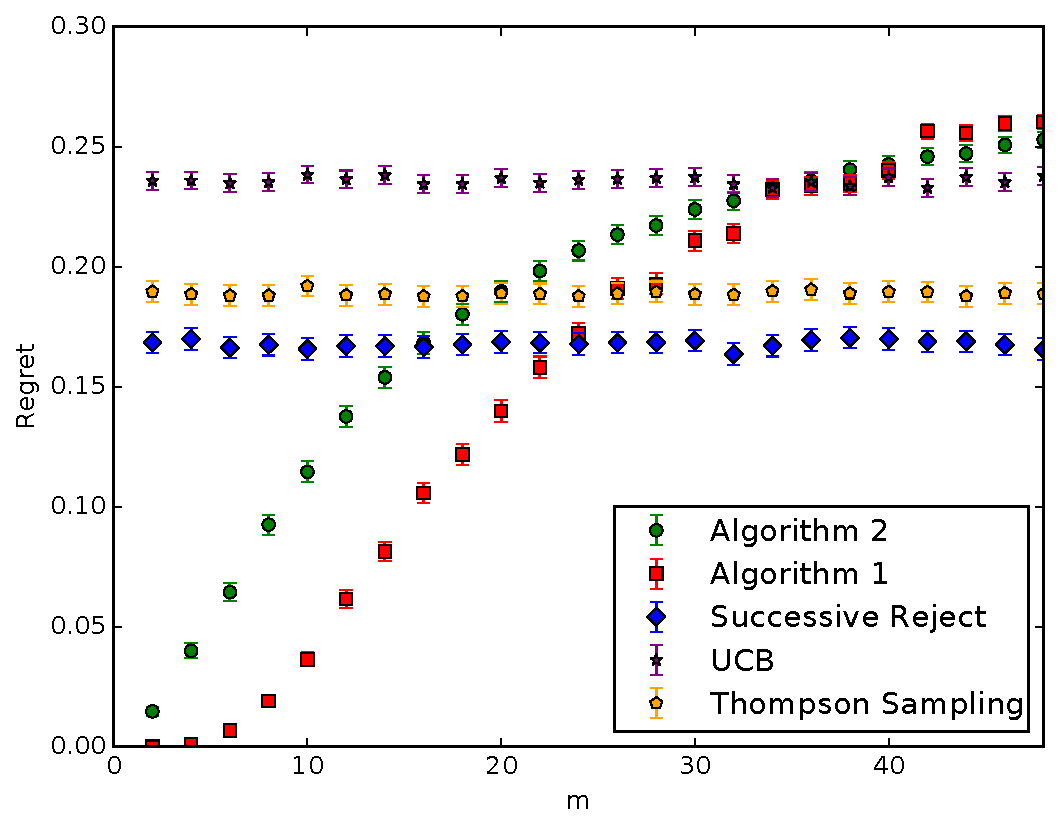
\includegraphics[width=\textwidth]{experiment1_20161020_1247.pdf}
    		\caption{Simple regret vs $m(\boldsymbol{q})$ for fixed horizon $T=400$ and number of variables $N = 50$}
        \label{fig:simple_vs_m}
    \end{subfigure}\hfill
    \begin{subfigure}[t]{0.3\textwidth}
    		\centering
        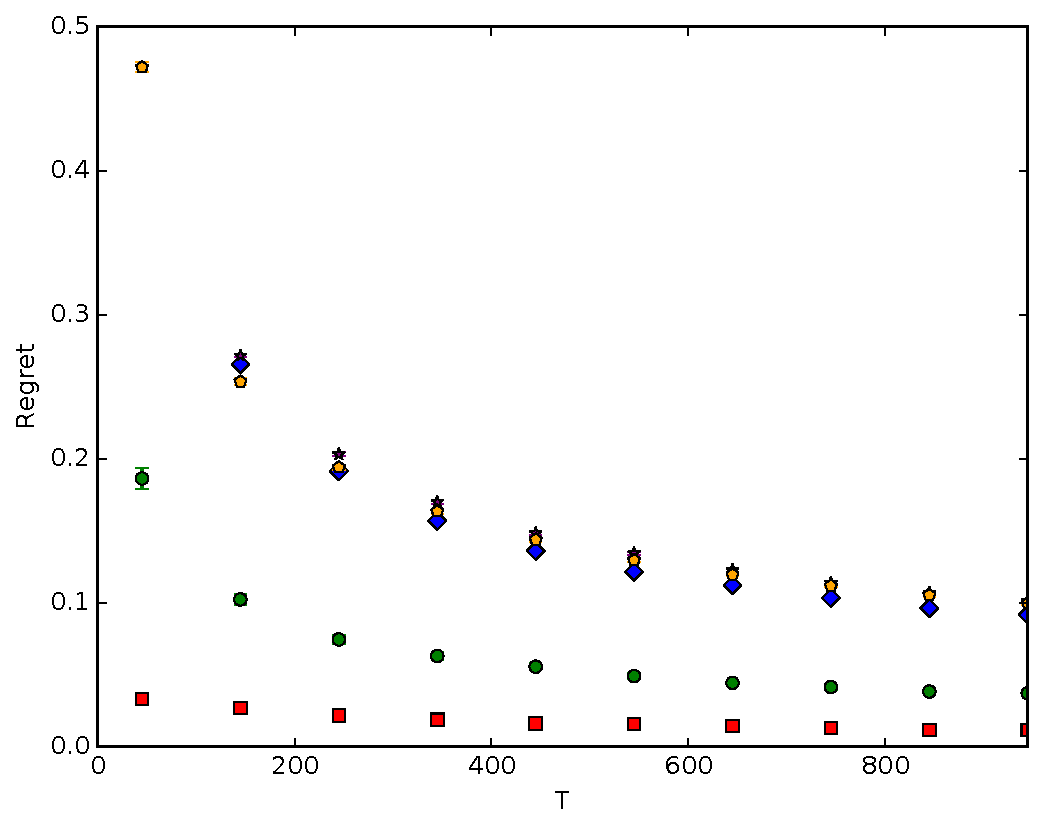
\includegraphics[width=\textwidth]{experiment2_20161020_1249.pdf}
    		\caption{Simple regret vs horizon, $T$, with $N = 50$, $m=2$ and $\epsilon = \sqrt{\frac{N}{8T}}$}
        \label{fig:simple_vs_T_vary_epsilon}
    \end{subfigure}\hfill
    \begin{subfigure}[t]{0.3\textwidth}
    		\centering
    		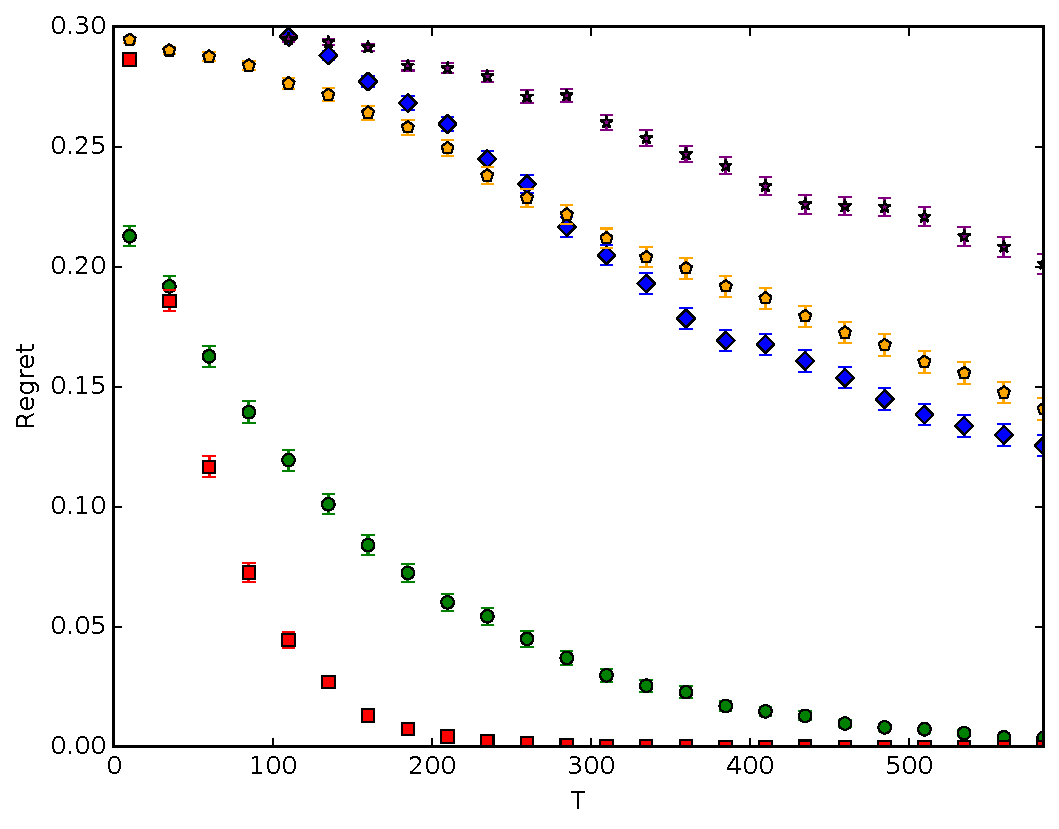
\includegraphics[width=\textwidth]{experiment3_20161020_1252.pdf}
    		\caption{Simple regret vs horizon, $T$, with $N = 50$, $m=2$ and fixed $\epsilon = .3$}
    		\label{fig:simple_vs_T}
    \end{subfigure}
    \caption{Experimental results}
    \label{fig:experiments}
\end{figure}

Figure \ref{fig:simple_vs_T_vary_epsilon} demonstrates the performance of the algorithms in the worst case environment for standard bandits, where the gap between the optimal and sub-optimal arms, $\smash{\epsilon = \sqrt{N/(8T)}}$ , is just too small to be learned. This gap is learn-able by the causal algorithms, for which the worst case $\epsilon$ depends on $m \ll N$. In Figure \ref{fig:simple_vs_T} we fix $N$ and $\epsilon$ and observe that, for sufficiently large $T$, the regret decays exponentially. The decay constant is larger for the causal algorithms as they have observed a greater effective number of samples for a given $T$. 

For the parallel bandit problem, the regression estimator used in the specific algorithm outperforms the truncated importance weighted estimator in the more general algorithm, despite the fact the specific algorithm must estimate $\boldsymbol{q}$ from the data. 
This is an interesting phenomenon that has been noted before in off-policy evaluation where the regression (and not the importance weighted) estimator is known to be mini-max optimal asymptotically \citep{li2014minimax}.


\begin{figure}[H]
	\centering    
          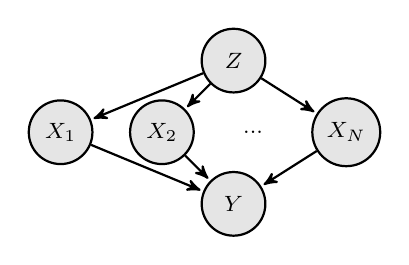
\begin{tikzpicture}[->,>=stealth',shorten >=1pt,auto,node distance=.45cm,
  thick,main node/.style={observed}, hidden/.style={empty},background rectangle/.style={fill=olive!45}]
%every node/.style={scale=0.6}
 %nodes
\node[main node](1){$X_{1}$};
\node[main node, right=of 1](2){$X_{2}$};
\node[hidden, right=of 2](3){$...$};
\node[main node, right=of 3](4){$X_{N}$};
\node[main node, below right=of 2](5){$Y$};
\node[main node, above right=of 2](6){$Z$};
 \path[every node/.style={font=\tiny}]
    (1) edge (5)
    	(2) edge (5)
    (4) edge (5)
    (6) edge (1) edge (2) edge (4);
\end{tikzpicture}
        \caption{Confounded graph}
        \label{fig:parallel_confounded} 
\end{figure}


We now compare the general algorithm with a range of standard bandit algorithms on the confounded graph in Figure \ref{fig:parallel_confounded}. All the variables are binary and the action space consists of the set of single variable interventions plus the do nothing action, 

\eq{
\calA = \set{\set{do(X_i = j)} \cup \set{do(Z = j)} \cup \set{do()}: 1\leq i \leq N,\; j \in \set{0,1}}
} 

We choose this setting because it generalises the parallel bandit, while simultaneously being sufficiently simple that we can compute the exact reward and interventional distributions for large $N$ (in general inference in graphical models is exponential in $N$). As before, we show the average regret over 10,000 simulations with error bars showing three standard errors. 

In Figure \ref{fig:simple_vs_m_general} we fix $N$ and $T$ and $P(Z=1) = .4$. For some $2 \leq N_1 \leq N$ we define 
\eq{
P(X_i = 1|Z = 0) &= \begin{cases} 0 & \text{ if } i \in \set{1,...N_1} \\ .4 & \text{ otherwise } \end{cases}\\
P(X_i = 1|Z = 1) &= \begin{cases} 0 & \text{ if } i \in \set{1,...N_1} \\ .65 & \text{ otherwise } \end{cases}
}
As in the parallel bandit case, we let $Y$ depend only on $X_1$, $P(Y|do(X_1=1)) = \frac{1}{2} + \epsilon$ and $P(Y|do(X_1=0)) = \frac{1}{2}-\epsilon'$, where $\epsilon' = \epsilon P(X_1=1) / P(X_1=0)$. The value of $N_1$ determines $m$ and ranges between $2$ and $N$. The values for the CPD's have been chosen such that the reward distribution is independent of $m$ and so that we can analytically calculate $\eta*$. This allows us to just show the dependence on $m$, removing the noise associated with different models selecting values for $\eta*$ with the same $m$ (and also worst case performance), but different performance for a given reward distribution. 

In Figure \ref{fig:simple_vs_T_general} we fix the model and number of variables, $N$, and vary the horizon $T$. $P(Z)$ and $P(X|Z)$ are the same as for the previous experiment.  
In Figure \ref{fig:simple_vs_T_misspecified} we additionally show the performance of Algorithm 1, but exclude actions on $Z$ from the set of allowable actions to demonstrate that Algorithm 1 can fail in the presence of a confounding variable, which occurs because it incorrectly assumes that $P(Y|do(X)) = P(Y|X)$. 
We let $P(Z) = .6$, $P(Y|\boldsymbol{X}) = X_7 \oplus X_N$ and $P(X|Z)$ be given by:

\eq{
P(X_i = 1|Z = 0) &= 
\begin{cases} 
.166 & \text{ if } i \in \set{1,..., 6} \\
.2 & \text{ if } i = 7 \\
.7 & \text { otherwise} 
 \end{cases}\\
 P(X_i = 1|Z = 1) &= 
\begin{cases} 
.166 & \text{ if } i \in \set{1,..., 6} \\
.8 & \text{ if } i = 7 \\
.3 & \text { otherwise} 
 \end{cases}\\
}

In this setting $X_7$ tends to agree with $Z$ and $X_N$ tends to disagree. It is sub-optimal to act on either $X_7$ or $X_N$, while all other actions are optimal. The first group of $X$ variables with $i \leq 6$ will be identified by the parallel bandit as the most unbalanced ones and played explicitly. All remaining variables are likely to be identified as balanced and estimated from observational estimates. The CPD values have been chosen to demonstrate the worst case outcome, where the bias in the estimates leads Algorithm 1 to asymptotically select a sub-optimal action.

\begin{figure}[H]
    \begin{subfigure}[t]{0.3\textwidth}
		\centering    
    		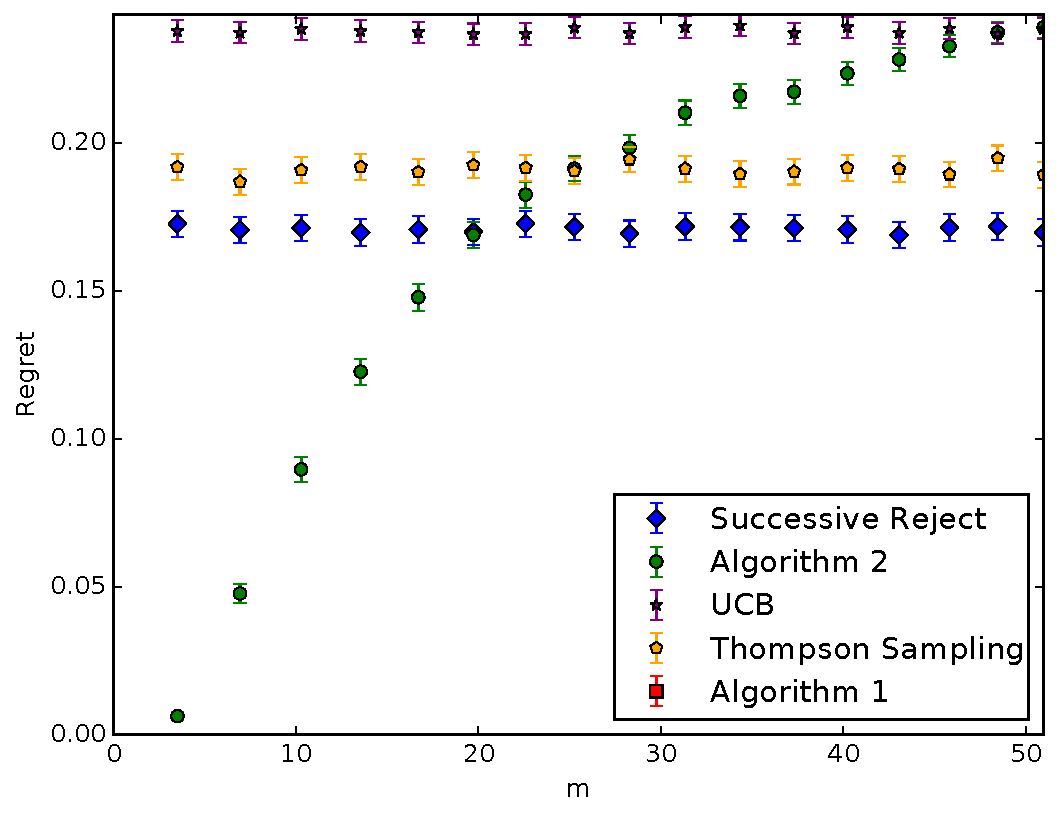
\includegraphics[width=\textwidth]{experiment4_20161023_2120.pdf}
    		\caption{Simple regret vs $m(\eta*)$ for fixed horizon $T=400$ and number of variables $N = 50$}
        \label{fig:simple_vs_m_general}
    \end{subfigure}\hfill
    \begin{subfigure}[t]{0.3\textwidth}
    		\centering
        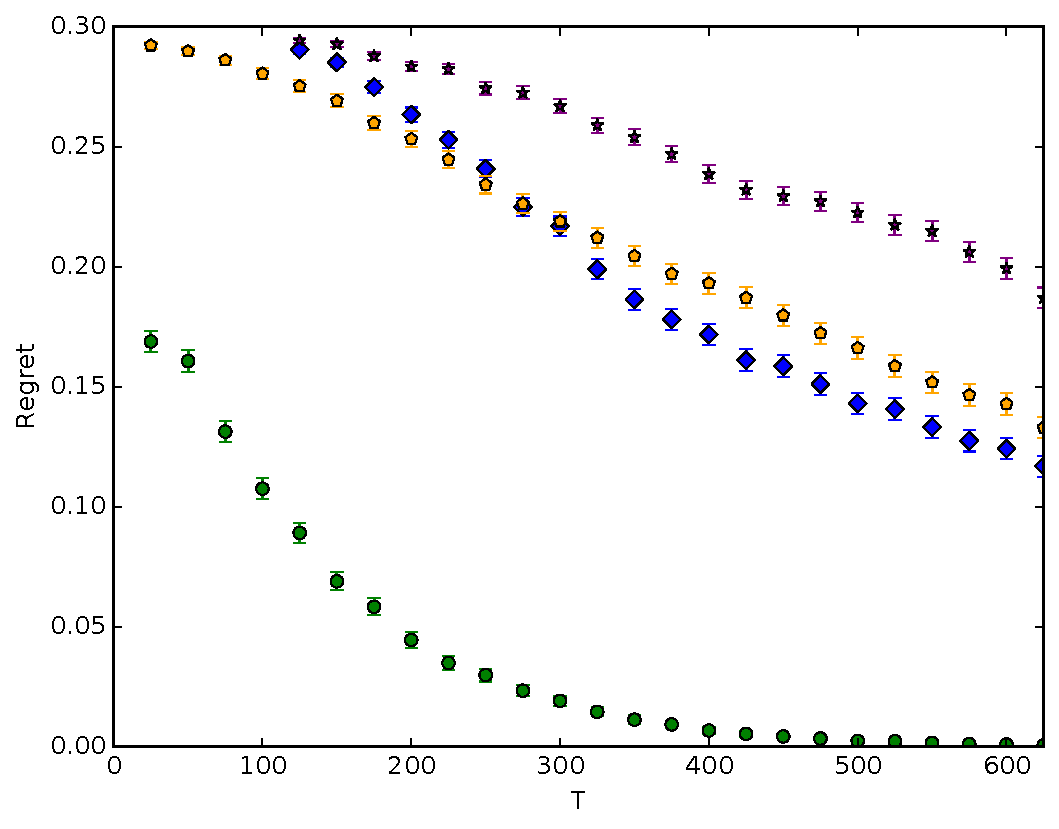
\includegraphics[width=\textwidth]{experiment7_20161020_1257.pdf}
    		\caption{Simple regret vs horizon, $T$, with $N = 50$ and $m(\eta*)=3.1$ }
        \label{fig:simple_vs_T_general}
    \end{subfigure}\hfill
    \begin{subfigure}[t]{0.3\textwidth}
    		\centering
    		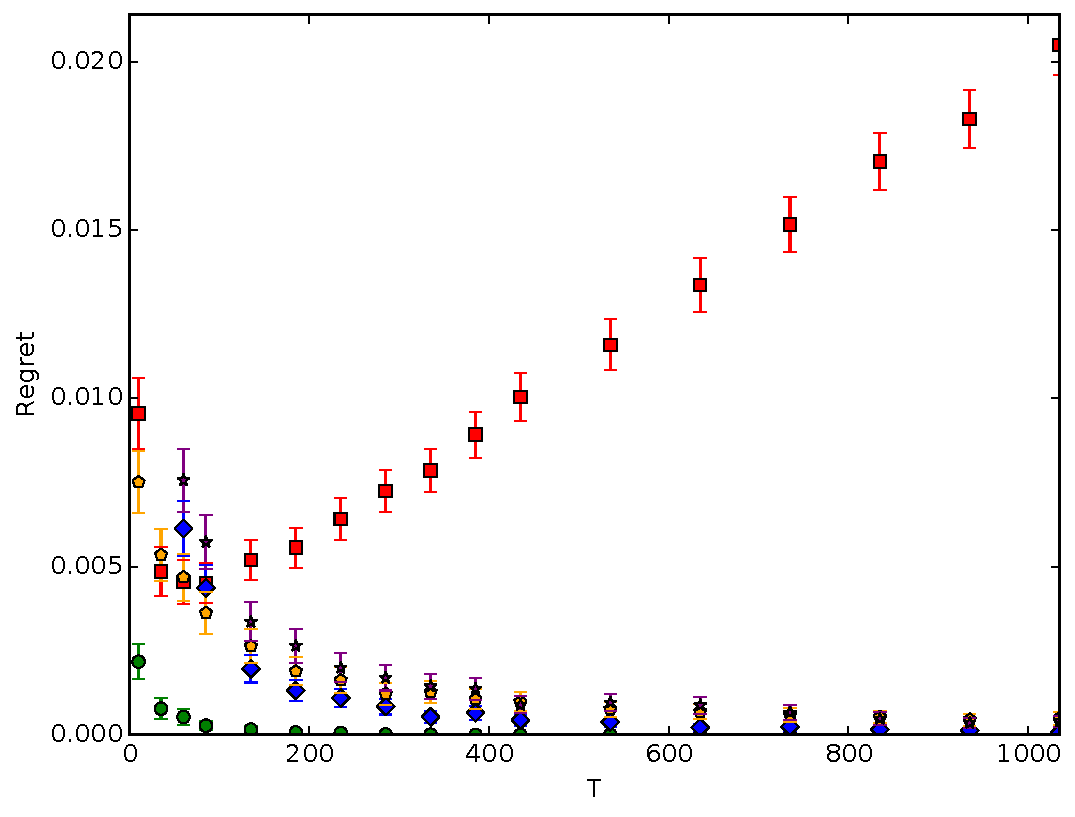
\includegraphics[width=\textwidth]{experiment5_20161023_2118.pdf}
    		\caption{Simple regret vs horizon, $T$, with $N = 21$, $m(\eta*)=4.3$ with no actions setting $Z$}
    		\label{fig:simple_vs_T_misspecified}
    \end{subfigure}
    \caption{Experimental results on the confounded graph}
    \label{fig:experiments_confounded}
\end{figure}

\subsection{Discussion \& Future work}
\label{sec:causal_bandit_discussion}
Algorithm~\ref{alg:general} for general causal bandit problems 
estimates the reward for all allowable interventions $a \in \calA$ over $T$ rounds by sampling and applying interventions from a distribution $\eta$.
Theorem~\ref{thm:general} shows that this algorithm has (up to log factors) simple regret that is $\smash{\mathcal O(\sqrt{m(\eta)/T)}}$ where 
the parameter $m(\eta)$ measures the difficulty of learning the causal model and is always less than $N$.
The value of $m(\eta)$ is a uniform bound on the variance of the reward estimators $\hat{\mu}_a$ and, intuitively, problems where all variables' values in the causal model ``occur naturally'' when interventions are sampled from $\eta$ will have low values of $m(\eta)$.

The main practical drawback of Algorithm~\ref{alg:general} is that both the estimator $\hat{\mu}_a$ and the optimal sampling distribution $\eta^*$ (\ie, the one that minimises $m(\eta)$) require knowledge of the conditional distributions $\Pn{a}{\parents{Y}}$ for all $a \in \calA$. In contrast, in the special case of parallel bandits, Algorithm~\ref{alg:simple} uses the $do()$ action to effectively estimate $m(\eta)$ and the rewards then re-samples the interventions with variances that are not bound by $\hat{m}(\eta)$.
Despite these extra estimates, Theorem~\ref{thm:lower} shows that this approach is optimal (up to log factors).Finding an algorithm that only requires the causal graph and lower bounds for its simple regret in the general case is left as future work.


\paragraph{Making Better Use of the Reward Signal}
Existing algorithms for best arm identification are based on ``successive rejection'' (SR) of arms based on UCB-like bounds on their rewards~\citep{Even-Dar2002}. In contrast, our algorithms completely ignore the reward signal when developing their arm sampling policies and only use the rewards when estimating $\hat{\mu}_a$. Incorporating the reward signal into our sampling techniques or designing more adaptive reward estimators that focus on high reward interventions is an obvious next step. This would likely improve the poor performance of our causal algorithm relative to the successive rejects algorithm for large $m$, as seen in Figure~\ref{fig:simple_vs_m}.

For the parallel bandit the required modifications should be quite straightforward. The idea would be to adapt the algorithm to essentially use successive elimination in the second phase so arms are eliminated as soon as they are provably no longer optimal with high probability. In the general case a similar modification is also possible by dividing the budget $T$ into phases and optimising the sampling distribution $\eta$, eliminating arms when their confidence intervals are no longer overlapping. This has now been done by \citet{Sen2017a}, leading to the first problem dependent regret bounds for causal bandit problems. Note that these modifications do not improve the mini-max regret, which at least for the parallel bandit is already optimal. For this reason we focused on emphasising the main point that causal structure can and should be exploited when available. Another observation is that Algorithm \ref{alg:general} is actually using a fixed design, which in some cases may be preferred to a sequential design for logistical reasons. This is not possible for Algorithm \ref{alg:simple}, since the $\vec{q}$ vector is unknown.


\paragraph{Cumulative Regret}
Although we have focused on simple regret in our analysis, it would also be natural to consider the cumulative regret. In the case of the parallel bandit problem we can slightly modify the analysis from \citep{wu2015online} on bandits with side information 
to get near-optimal cumulative regret guarantees. They consider a finite-armed bandit model with side information where in reach round the learner chooses an action and receives a Gaussian reward signal for all actions, but with a known variance that depends on the chosen action. In this way the learner can gain information about actions it does not take with varying levels of accuracy. The reduction follows by substituting the importance weighted estimators in place of the Gaussian reward. In the case that $\vec{q}$ is known this would lead to a known variance and the only (insignificant) difference is the Bernoulli noise model. In the parallel bandit case we believe this would lead to near-optimal cumulative regret,
at least asymptotically. 

%Their model assumes the rewards for all arms $a$ are Gaussian with mean $\mu_a$ and variance $\sigma^2_{ab}$ and that playing an arm $a$ will reveal a side observation $Y_{ab}$ of the reward for all arms $b$ distributed with mean $\mu_b$ and variance $\sigma^2_{ab}$.
%We can build a similar dependence structure with variances for a Bernoulli reward variable that is derived from the $\vec{q}$ vector of probabilities.
%\todom{Check this!}
%Even though the original results are for Gaussian rewards we believe the analysis will go through largely unchanged.

The parallel bandit problem can also be viewed as an instance of a time varying graph feedback problem \citep{Alon2015,Kocak2014}, where at each time step the feedback graph $G_t$ is selected stochastically, dependent on $\boldsymbol{q}$, and revealed after an action has been chosen. The feedback graph is distinct from the causal graph. A link $A \rightarrow B$ in $G_t$ indicates that selecting the action $A$ reveals the reward for action $B$. For this parallel bandit problem, $G_t$ will always be a star graph with the action $do()$ connected to half the remaining actions. However, \citet{Alon2015,Kocak2014} give adversarial algorithms, which when applied to the parallel bandit problem obtain the standard bandit regret. A malicious adversary can select the same graph each time, such that the rewards for half the arms are never revealed by the informative action. This is equivalent to a nominally stochastic selection of feedback graph where $\boldsymbol{q} = \boldsymbol{0}$. 

\citet{Lelarge2012} consider a stochastic version of the graph feedback problem, but with a fixed graph available to the algorithm before it must select an action. In addition, their algorithm is not optimal for all graph structures and fails, in particular, to provide improvements for star like graphs as in our case. \citep{Buccapatnam2014} improve the dependence of the algorithm on the graph structure but still assume the graph is fixed and available to the algorithm before the action is selected. 



\paragraph{Causal Models with Non-Observable Variables}
If we assume knowledge of the conditional \textit{interventional} distributions $\Pn{a}{\parents{Y}}$ our analysis applies unchanged to the case of causal models with 
non-observable variables. Some of the interventional distributions may be non-identifiable meaning we can not obtain prior estimates for $\Pn{a}{\parents{Y}}$ from 
even an infinite amount of observational data. Even if all variables are observable and the graph is known, if the conditional distributions are unknown, then Algorithm
\ref{alg:general} cannot be used. Estimating these quantities while simultaneously minimising the simple regret is an interesting and challenging open problem.

% For example, if we had access to a data set of \textit{experiments} in which the reward variable $Y$ was not available from which to build estimates of $P_a$.
% In this case, some conditional distributions may be non-identifiable. 
% The corresponding actions can be immediately added to the set $A$ prior to collecting any data. 
% We can then use the same algorithm as in the case where there are no latent variables, except that we will have to use the more general do-calculus rather than simply adjusting for the parents to write the expression for each action in terms of observational data.
% Combining our estimation techniques with insights from \citet{Bareinboim2015} for handling unobserved confounders would be worth investigation.


% More generally, assuming causal structure creates more complex types of side information, such as that shown in equation \ref{eq:estimation_transfer}. In this case, selecting one action does not fully reveal an alternate action but provides some information towards an estimate. The quality of the estimate notably depends not only on the number of times that action was selected. For example, to get a good estimate for $X_1 = 1$ by intervening on $X_2$ requires us to sample both $X_2=0$ and $X_2=1$, in proportions dependent on $q_2$. This more complex side information does not fit within the graph feedback framework.


\paragraph{Partially or Completely Unknown Causal Graph}
A much more difficult generalisation would be to consider causal bandit problems where the causal graph is completely unknown or known to be a member of class of models.
The latter case arises naturally if we assume free access to a large observational data set, from which the Markov equivalence class can be found via causal discovery techniques. 
Work on the problem of selecting experiments to discover the correct causal graph from within a Markov equivalence class~\citep{eberhardt2005,eberhardt2010causal,hauser2014two,Hu2014} could potentially be incorporated into a causal bandit algorithm.
In particular, \citet{Hu2014} show that only $\bigo{\log \log n}$ multi-variable interventions are required on average to recover a causal graph over $n$ variables once purely observational data is used to recover the ``essential graph''.
Simultaneously learning a completely unknown causal model while estimating the rewards of interventions without a large observational data set would be much more challenging.

\subsection{Proofs}
\subsubsection{Proof of Theorem \ref{thm:uq-simple}}\label{sec:thm:uq-simple}


Assume without loss of generality that $q_1 \leq q_2 \leq \ldots \leq q_N \leq 1/2$. The assumption is non-restrictive since all variables
are independent and permutations of the variables can be pushed to the reward function. 

The proof of Theorem \ref{thm:uq-simple} requires some lemmas. \

\begin{lemma}\label{lem:conc1}
Let $i \in \set{1,\ldots, N}$ and $\delta > 0$. Then
\eq{
\P{\left|\hat q_i - q_i\right| \geq \sqrt{\frac{6q_i}{T} \log \frac{2}{\delta}}} \leq \delta\,.
}
\end{lemma}

\begin{proof}
By definition, $\hat{q}_i = \frac{2}{T}\sum_{t=1}^{T/2}X_{t,i}$, where $X_{t,i} \sim Bernoulli(q_i)$. Therefore from the Chernoff bound (see equation 6 in \citet{Hagerup1990}),

\eq{
\P{\left|\hat q_i - q_i\right| \geq \epsilon} \leq 2e^{-\frac{T\epsilon^2}{6q_i}}
}

Letting $\delta = 2e^{-\frac{T\epsilon^2}{6q_i}}$ and solving for $\epsilon$ completes the proof.

\end{proof}

\begin{lemma}\label{lem:m_est}

Let $\delta \in (0,1)$ and assume $T \geq 48m \log\frac{2N}{\delta}$. Then
\eq{
\P{2m(\vec{q}) / 3 \leq m(\vec{\hat q}) \leq 2m(\vec{q})} \geq 1 - \delta\,.
}
\end{lemma}

\begin{proof}
Let $F$ be the event that there exists and $1 \leq i \leq N$ for which
\eq{
\left|\hat q_i - q_i\right| \geq \sqrt{\frac{6q_i}{T} \log \frac{2N}{\delta}}\,.
}
Then by the union bound and Lemma \ref{lem:conc1} we have $\P{F} \leq \delta$. The result will be completed by showing that
when $F$ does not hold we have $2m(\vec{q})/3 \leq m(\vec{\hat q}) \leq 2m(\vec{q})$.
From the definition of $m(\vec{q})$ and our assumption on $\vec{q}$ we have for $i > m(\vec{q})$ that $q_i \geq q_m \geq 1/m(\vec{q})$ and so by Lemma \ref{lem:conc1} we have
\eq{
\frac{3}{4} 
&\geq \frac{1}{2} + \sqrt{\frac{3}{T} \log \frac{2N}{\delta}} 
\geq q_i + \sqrt{\frac{6q_i}{T} \log \frac{2N}{\delta}} 
\geq \hat q_i \\
&\geq q_i - \sqrt{\frac{6q_i}{T} \log \frac{2N}{\delta}}
\geq q_i - \sqrt{\frac{q_i}{8m(\vec{q})}}
\geq \frac{1}{2m(\vec{q})}\,.
}
Therefore by the pigeonhole principle we have $m(\vec{\hat q}) \leq 2m(\vec{q})$.
For the other direction we proceed in a similar fashion. Since the failure event $F$ does not hold we have for $i \leq m(\vec{q})$ that
\eq{
\hat q_i 
\leq q_i + \sqrt{\frac{6q_i}{T} \log\frac{2N}{\delta}} 
\leq \frac{1}{m(\vec{q})} \left(1 + \sqrt{\frac{1}{8}}\right)
\leq \frac{3}{2m(\vec{q})}\,.
}
Therefore $m(\vec{\hat q}) \geq 2m(\vec{q}) / 3$ as required. 
\end{proof}

\begin{proof}[Proof of Theorem \ref{thm:uq-simple}]
Recall that $A = \set{a \in \actions : \hat p_a \leq 1/m(\vec{\hat q})}$. Then,
for $a \in A$, the algorithm estimates $\mu_a$ from $T_A \doteq T/(2m(\vec{\hat q}))$ samples. From lemma \ref{lem:m_est}, $T_A  \geq T/(4m(\vec{q}))$ with probability $(1-\delta)$. Let $H$ be the event $T_A < T/(4m(\vec{q}))$ and $G$ be the event $\exists a \in A : |\mu_a - \hat \mu_a| \geq \sqrt{\frac{2m(\vec{q})}{T} \log\frac{2N}{\delta}}$

\eq{
\P{G} \leq \P{H} + \P{G|\neg H} \leq \delta + \P{G|\neg H}
}

Via Hoeffding's inequality and the union bound, 

\eq{
\P{G|\neg H}&\doteq \P{\exists a \in A : |\mu_a - \hat \mu_a| \geq \sqrt{\frac{2m(\vec{q})}{T} \log\frac{2N}{\delta}},\text{ given }T_A \geq T/(4m(\vec{q}))} \leq \delta\\
 \implies  \P{G} & \doteq \P{\exists a \in A : |\mu_a - \hat \mu_a| \geq \sqrt{\frac{2m(\vec{q})}{T} \log\frac{2N}{\delta}}} \leq 2\delta\,.
}
For arms not in $A$,

\eq{
\hat p_a = & \frac{2}{T} \sum_{t=1}^{T/2} \ind{X_i = j} \geq 1/m(\vec{\hat q}), \; \text {by definition of not being in $A$}\\
 \geq & \frac{1}{2m(\vec{q})},\; \text{ with probability } 1-\delta \\
\implies  T_a \doteq & \sum_{t=1}^{T/2} \ind{X_i = j} \geq  \frac{T}{4m(\vec{q})},\; \text{ with probability } 1-\delta
}

Again applying Hoeffding's and the union bound

\eq{
\P{\exists a \notin A:  \left|\hat \mu_a - \mu_a\right| \geq \sqrt{\frac{2m(\vec{q})}{T} \log \frac{2N}{\delta}}} \leq 2\delta
}


Therefore, combining this result with the bound for arms $a \in A$, we have with probability at least $1 - 4\delta$ that,
\eq{
(\forall a \in \actions) \qquad |\hat \mu_a - \mu_a| \leq \sqrt{\frac{2m(\vec{q})}{T} \log \frac{2N}{\delta}} \doteq \epsilon\,.
}
If this occurs, then 
\eq{
\mu_{\hat a^*_T} \geq \hat \mu_{\hat a^*_T} - \epsilon \geq \hat \mu_{a^*} - \epsilon \geq \mu_{a^*} - 2\epsilon\,.
}
Therefore
\eq{
\mu^* - \EE[\mu_{\hat a^*_T}] 
& \leq 4\delta + \epsilon\\
& \leq \frac{8m(\vec{q})}{T} + \sqrt{\frac{2m(\vec{q})}{T} \log \frac{NT}{m(\vec{q})}},\; \text{ letting } \delta = \frac{2m(\vec{q})}{T}\\
& \leq \sqrt{\frac{20m(\vec{q})}{T} \log \frac{NT}{m(\vec{q})}},\; \text{ via Jenson's Inequality}
}
which completes the result.
\end{proof}

%%%%%%%%%%%%%%%%%%%%%%%%%%%%%%%%%%%%%%%%%%%%
% LOWER BOUND
%%%%%%%%%%%%%%%%%%%%%%%%%%%%%%%%%%%%%%%%%%%%
\subsubsection{Proof of Theorem \ref{thm:lower}}\label{sec:thm:lower}

We follow a relatively standard path by choosing multiple environments that have different optimal arms, but which cannot all be statistically
separated in $T$ rounds.
Assume without loss of generality that $q_1 \leq q_2 \leq \ldots \leq q_N \leq 1/2$.
For each $i$ define reward function $r_i$ by
\eq{
r_0(\boldsymbol{X}) &= \frac{1}{2} &
r_i(\boldsymbol{X}) &= \begin{cases}
\frac{1}{2} + \epsilon & \text{if } X_i = 1 \\
\frac{1}{2} & \text{otherwise}\,,
\end{cases}
}
where $1/4 \geq \epsilon > 0$ is some constant to be chosen later.
We abbreviate $R_{T,i}$ to be the expected simple regret incurred when interacting with the
environment determined by $\boldsymbol{q}$ and $r_i$. Let $\operatorname{P}_i$ be the corresponding measure
on all observations over all $T$ rounds and $\EE_i$ the expectation with respect to $\operatorname{P}_i$. By Lemma 2.6 by \citet{Tsy08} we have
\eq{
\Prz{\hat a^*_T = a^*} + \Pri{\hat a^*_T \neq a^*} \geq \exp\left(-\KL(\operatorname{P}_0, \operatorname{P}_i)\right)\,,
}
where $\KL(\Ps_0, \Ps_i)$ is the KL divergence between measures $\operatorname{P}_0$ and $\operatorname{P}_i$.
Let $T_i(T) = \sum_{t=1}^T \ind{a_t = do(X_i = 1)}$ be the total number of times the learner intervenes on variable $i$ by setting it to $1$.
Then for $i \leq m$ we have $q_i \leq 1/m$ and the KL divergence between $\Ps_0$ and $\Ps_i$ may be bounded using the telescoping property (chain rule) and
by bounding the local KL divergence by the $\chi$-squared distance as by \citet{Auer1995}. This leads to 
\eq{
\KL(\Ps_0, \Ps_i) 
&\leq 6\epsilon^2 \EE_0\left[\sum_{t=1}^T \ind{X_{t,i} = 1}\right] 
\leq 6\epsilon^2 \left(\EE_0 T_i(T) + q_i T\right) 
\leq 6\epsilon^2 \left(\EE_0 T_i(T) + \frac{T}{m}\right)\,.
}
Define set $A = \set{i \leq m : \EE_0 T_i(T) \leq 2T / m}$.
Then for $i \in A$ and choosing $\epsilon = \min\set{1/4, \sqrt{m/(18T)}}$ we have
\eq{
\KL(\Ps_0, \Ps_i) \leq \frac{18T\epsilon^2}{m} = 1\,. 
}
Now $\sum_{i=1}^m \EE_0 T_i(T) \leq T$, which implies that $|A| \geq m/2$.
Therefore
\eq{
\sum_{i \in A} \Pri{\hat a^*_T \neq a} 
\geq \sum_{i \in A} \exp\left(-\KL(\Ps_0, \Ps_i)\right) - 1
\geq \frac{|A|}{e} - 1 
\geq \frac{m}{2e} - 1\,.
}
Therefore there exists an $i \in A$ such that
$\Pri{\hat a^*_T \neq a^*} \geq \frac{\frac{m}{2e} - 1}{m}$. 
Therefore if $\epsilon < 1/4$ we have
\eq{
R_{T,i} \geq \frac{1}{2} \Pn{i}{\hat a^*_T \neq a^*} \epsilon \geq \frac{\frac{m}{2e} - 1}{2m} \sqrt{\frac{m}{18T}}\,.
}
Otherwise $m \geq 18T$ so $\sqrt{m/T} = \Omega(1)$ and
\eq{
R_{T,i} \geq \frac{1}{2} \Pn{i}{\hat a^*_T \neq a^*} \epsilon \geq \frac{1}{4} \frac{\frac{m}{2e} - 1}{2m} \in \Omega(1) 
}
as required.

%%%%%%%%%%%%%%%%%%%%%%%%%%%%%%%%%%%%%%%%%%%%
% GENERAL-GRAPH UPPER BOUND
%%%%%%%%%%%%%%%%%%%%%%%%%%%%%%%%%%%%%%%%%%%%
\subsubsection{Proof of Theorem \ref{thm:general}}\label{sec:thm:general}

\begin{proof}
First note that $X_t, Y_t$ are sampled from $\operatorname{Q}$.
We define $Z_a(X_t) = Y_t R_a(X_t)\ind{R_a(X_t)\leq B_a}$ and abbreviate $Z_{at} = Z_a(X_t)$, $R_{at} = R_a(X_t)$ and $\Pn{a}{.} = \Pns{a}{.}$.
By definition we have $|Z_{at}| \leq B_a$ and 
\eq{
\Var_Q[Z_{at}] 
\leq \EE_Q[Z_{at}^2] 
\leq \EE_Q[R_{at}^2]
= \EEa[R_{at}]
= \EEa\left[\frac{\Pns{a}{\parents{Y}(X)}}{\Q{\parents{Y}(X)}}\right] 
\leq m(\eta)\,.
}
Checking the expectation we have
\eq{
\EE_Q[Z_{at}] 
= \EEa \left[Y \ind{R_{at} \leq B_a}\right] 
= \EEa Y - \EEa \left[Y\ind{R_{at} > B_a}\right] 
= \mu_a - \beta_a\,,
}
where 
\eq{
0 \leq \beta_a = \EEa[Y \ind{R_{at} > B_a}] \leq \Pns{a}{R_{at} > B_a}
}
is the negative bias. 
The bias may be bounded in terms of $m(\eta)$ via an application of Markov's inequality.
\eq{
\beta_a \leq \Pns{a}{R_{at} > B_a} \leq \frac{\EEa[R_{at}]}{B_a} \leq \frac{m(\eta)}{B_a}\,.
}
Let $\epsilon_a > 0$ be given by
\eq{
\epsilon_a = \sqrt{\frac{2m(\eta)}{T} \log\left(2T|\calA|\right)} + \frac{3B_a}{T} \log\left(2T|\calA|\right)\,.
}
Then by the union bound and Bernstein's inequality 
\eq{
\P{\text{exists } a \in \calA : \left|\hat \mu_a - \EE_Q[Z_{at}]\right| \geq \epsilon_a} 
\leq \sum_{a \in \calA} \P{\left|\hat \mu_a - \EE_Q[Z_{at}]\right| \geq \epsilon_a} \leq \frac{1}{T}\,.
}

Let $I = \hat{a}^*_T$ be the action selected by the algorithm, $a^* = \argmax_{a \in \calA} \mu_a$ be the true optimal action and recall that $\EE_Q[Z_{at}] = \mu_a - \beta_a$. Assuming the above event does not occur we have,

\eq{
\mu_I \geq \hat \mu_I - \epsilon_I  
\geq \hat \mu_{a^*} - \epsilon_I  
\geq \mu^* - \epsilon_{a^*} - \epsilon_I - \beta_{a^*}\,. 
}
By the definition of the truncation
we have
\eq{
\epsilon_a \leq \left(\sqrt{2} + 3\right)\sqrt{\frac{m(\eta)}{T} \log\left(2T|\calA|\right)}
}
and
\eq{
\beta_a \leq \sqrt{\frac{m(\eta)}{T} \log\left(2T|\calA|\right)}\,. 
}
Therefore for $C = \sqrt{2} + 4$ we have
\eq{
\P{\mu_I \geq \mu^* - C \sqrt{\frac{m(\eta)}{T} \log\left(2T|\calA|\right)}} \leq \frac{1}{T}\,.
}
Therefore
\eq{
\mu^* - \EE[\mu_I] \leq C \sqrt{\frac{m(\eta)}{T} \log\left(2T|\calA|\right)} + \frac{1}{T}
}
as required.
\end{proof}

\subsubsection{Relationship between $m(\eta)$ and $m(\boldsymbol{q})$}\label{sec:m-equivelence}

\begin{proposition} In the parallel bandit setting,
$m(\eta^*) \leq 2m(\boldsymbol{q})$.
\end{proposition} 

\begin{proof}

Recall that in the parallel bandit setting,

\eq{
\mathcal{A} = \set{do()} \cup \set{ do(X_i = j) \colon 1 \leq i \leq N \text{ and } j \in \set{0,1}}
}

Let:

\eq {
\eta_a = \ind{\P{X_i = j} < \frac{1}{m(\boldsymbol{q})}}\frac{1}{2m(\boldsymbol{q})} \text { for } a \in do(X_i = j)
}

Let $D =\sum_{a\in do(X_i=j)}\eta_a$. From the definition of $m(\boldsymbol{q})$, 
\eq {
\sum_{a\in do(X_i=j)} \ind{\P{X_i = j} < \frac{1}{m(\boldsymbol{q})}} \leq m(\boldsymbol{q}) \implies D \leq \frac{1}{2}
}
 
Let $\eta_a = \frac{1}{2} + (1-D)$ for $a = do()$ such that $\sum_{a \in \calA}\eta_a = 1$ 

Recall that,

\eq{
m(\eta) &
= \max_a \EEa\left[\frac{\Pn{a}{\parents{Y}(X)}}{\Q{\parents{Y}(X)}}\right]
}

We now show that our choice of $\eta$ ensures $\EEa\left[\frac{\Pn{a}{\parents{Y}(X)}}{\Q{\parents{Y}(X)}}\right] \leq 2m(\boldsymbol{q})$ for all actions $a$.

For the actions $a: \eta_a > 0$, ie $do()$ and $do(X_i = j):\P{X_i=j}<\frac{1}{m(\boldsymbol{q})}$,
\eq{
\EEa\left[\frac{\Pn{a}{X_1...X_N}}{\sum_{b}\eta_b\Pn{b}{X_1...X_N}}\right] \leq \EEa\left[\frac{\Pn{a}{X_1...X_N}}{\eta_a\Pn{a}{X_1...X_N}}\right] = \EEa\left[\frac{1}{\eta_a}\right] \leq 2m(\boldsymbol{q})
}

For the actions $a :\eta_a = 0$, ie $do(X_i=j):\P{X_i=j}\geq\frac{1}{m(\boldsymbol{q})}$,
\eq{
\EEa\left[\frac{\Pn{a}{X_1...X_N}}{\sum_{b}\eta_b\Pn{b}{X_1...X_N}}\right] \leq & \EEa\left[\frac{\ind{X_i=j}\prod_{k\neq i}\P{X_k}}{(1/2+D)\prod_k \P{X_k}}\right] \\=& \EEa\left[\frac{\ind{X_i=j}}{(1/2+D)\P{X_i = j}}\right]
\leq  \EEa\left[\frac{\ind{X_i=j}}{(1/2)(1/m(\boldsymbol{q}))}\right] \leq 2m(\boldsymbol{q})
}

Therefore $m(\eta*) \leq m(\eta) \leq 2m(\boldsymbol{q})$ as required.

\end{proof}

{\small\bibliography{library}}
\bibliographystyle{apalike}
\end{document}
